\documentclass[aspectratio=169,12pt,t]{beamer}

% --- Theme: Metropolis (modern, clean) ---
\usetheme[progressbar=frametitle,numbering=fraction,block=fill]{metropolis}

% --- Fira Sans font (install texlive-fonts-extra if missing) ---
\IfFileExists{FiraSans.sty}{\usepackage[sfdefault]{FiraSans}}{}

% --- Light background with warm accent ---
\definecolor{mDarkTeal}{RGB}{35,55,59}
\definecolor{mLightBrown}{RGB}{235,228,216}
\definecolor{mAccent}{RGB}{140,70,20}

\setbeamercolor{normal text}{fg=mDarkTeal,bg=white}
\setbeamercolor{alerted text}{fg=mAccent}
\setbeamercolor{frametitle}{bg=mDarkTeal,fg=white}
\setbeamercolor{progress bar}{fg=mAccent,bg=mLightBrown}
\setbeamercolor{title separator}{fg=mAccent}
\setbeamercolor{progress bar in head/foot}{fg=mAccent,bg=mLightBrown}
\setbeamercolor{progress bar in section page}{fg=mAccent,bg=mLightBrown}

% --- Packages ---
\usepackage[utf8]{inputenc}
\usepackage{amsmath,amssymb,amsthm}
\usepackage{mathrsfs}
\usepackage{tikz}
\usetikzlibrary{arrows.meta,positioning,calc,decorations.pathreplacing,shapes,patterns}
\usepackage{pgfplots}
\pgfplotsset{compat=1.18}
\usepgfplotslibrary{fillbetween}

% --- TikZ diagram styles (shared across the series) ---
\tikzset{
  axisln/.style={-{Stealth[length=2.6mm]}, line width=0.8pt, gray!75},
  curveln/.style={line width=1.6pt, line cap=round, line join=round},
  projln/.style={dash pattern=on 2.6pt off 2pt, line width=0.7pt},
  guide/.style={-{Stealth[length=2.6mm,width=2.2mm]}, line width=1.1pt},
  box/.style={draw=#1, fill=#1!12, line width=1pt, rounded corners=2pt,
    minimum width=5.6cm, minimum height=1.35cm, align=center, font=\small},
}
% point marker with a white halo: \dotpt{color}{(coord)}
\newcommand{\dotpt}[2]{%
  \fill[white] #2 circle (3.6pt);
  \fill[#1] #2 circle (2.4pt);
}
% open point marker: \opendotpt{color}{(coord)}
\newcommand{\opendotpt}[2]{%
  \fill[white] #2 circle (3.6pt);
  \draw[#1, line width=1pt] #2 circle (2.4pt);
}

% --- Semi-transparent white highlight for text on top of background images ---
\usepackage[most]{tcolorbox}

% Inline highlight: \hl{short text}
\newtcbox{\hl}{%
  nobeforeafter, tcbox raise base,
  colback=white, opacityback=0.6,
  colframe=white, opacityframe=0,
  sharp corners, boxsep=2pt, left=3pt, right=3pt, top=2pt, bottom=2pt%
}

% Block highlight: \begin{hlbox} ... \end{hlbox}  (multi-line, paragraphs, itemize)
% Optional argument accepts any tcolorbox key, e.g. [width=0.6\linewidth]
\newtcolorbox{hlbox}[1][]{%
  enhanced, breakable,
  colback=white, opacityback=0.6,
  colframe=white, opacityframe=0,
  boxsep=3pt, left=6pt, right=6pt, top=4pt, bottom=4pt,
  sharp corners,
  {#1}%
}

% --- Custom colors for content types ---
\definecolor{defcolor}{RGB}{25,85,120}
\definecolor{thmcolor}{RGB}{140,35,35}
\definecolor{proofcolor}{RGB}{35,100,50}
\definecolor{excolor}{RGB}{140,75,10}
\definecolor{remcolor}{RGB}{90,90,90}

% --- Beamer blocks for mathematical content types (semi-transparent) ---
\tcbset{hlblockbase/.style={
  enhanced, breakable,
  coltitle=white, fonttitle=\bfseries,
  opacitybacktitle=0.8, opacityback=0.6,
  opacityframe=0,
  sharp corners,
  boxsep=1pt, left=5pt, right=5pt, top=2pt, bottom=2pt,
  toptitle=1pt, bottomtitle=1pt,
  before upper={\setlength{\abovedisplayskip}{4pt}\setlength{\belowdisplayskip}{4pt}}
}}

\newtcolorbox{defblock}[1]{hlblockbase, title={#1},
  colbacktitle=defcolor, colback=defcolor!15, colframe=defcolor}
\newtcolorbox{thmblock}[1]{hlblockbase, title={#1},
  colbacktitle=thmcolor, colback=thmcolor!15, colframe=thmcolor}
\newtcolorbox{proofblock}[1]{hlblockbase, title={#1},
  colbacktitle=proofcolor, colback=proofcolor!15, colframe=proofcolor}
\newtcolorbox{exblock}[1]{hlblockbase, title={#1},
  colbacktitle=excolor, colback=excolor!15, colframe=excolor}
\newtcolorbox{remblock}[1]{hlblockbase, title={#1},
  colbacktitle=remcolor, colback=remcolor!15, colframe=remcolor}

% --- Metadata ---
\title{Chapter 7: Sequences and Series of Functions}
\subtitle{Section: Uniform Convergence and Continuity}
\author{Based on Walter Rudin's \emph{Principles of Mathematical Analysis}}
\date{}

% --- Shared plot helpers for this deck ---
% Dini example: g_n(x) = 4 x^n (1 - x) decreases to 0 on [0,1]
\pgfmathdeclarefunction{dinig}{2}{\pgfmathparse{4*(#1)^(#2)*(1-(#1))}}

\begin{document}

{
\usebackgroundtemplate{%
  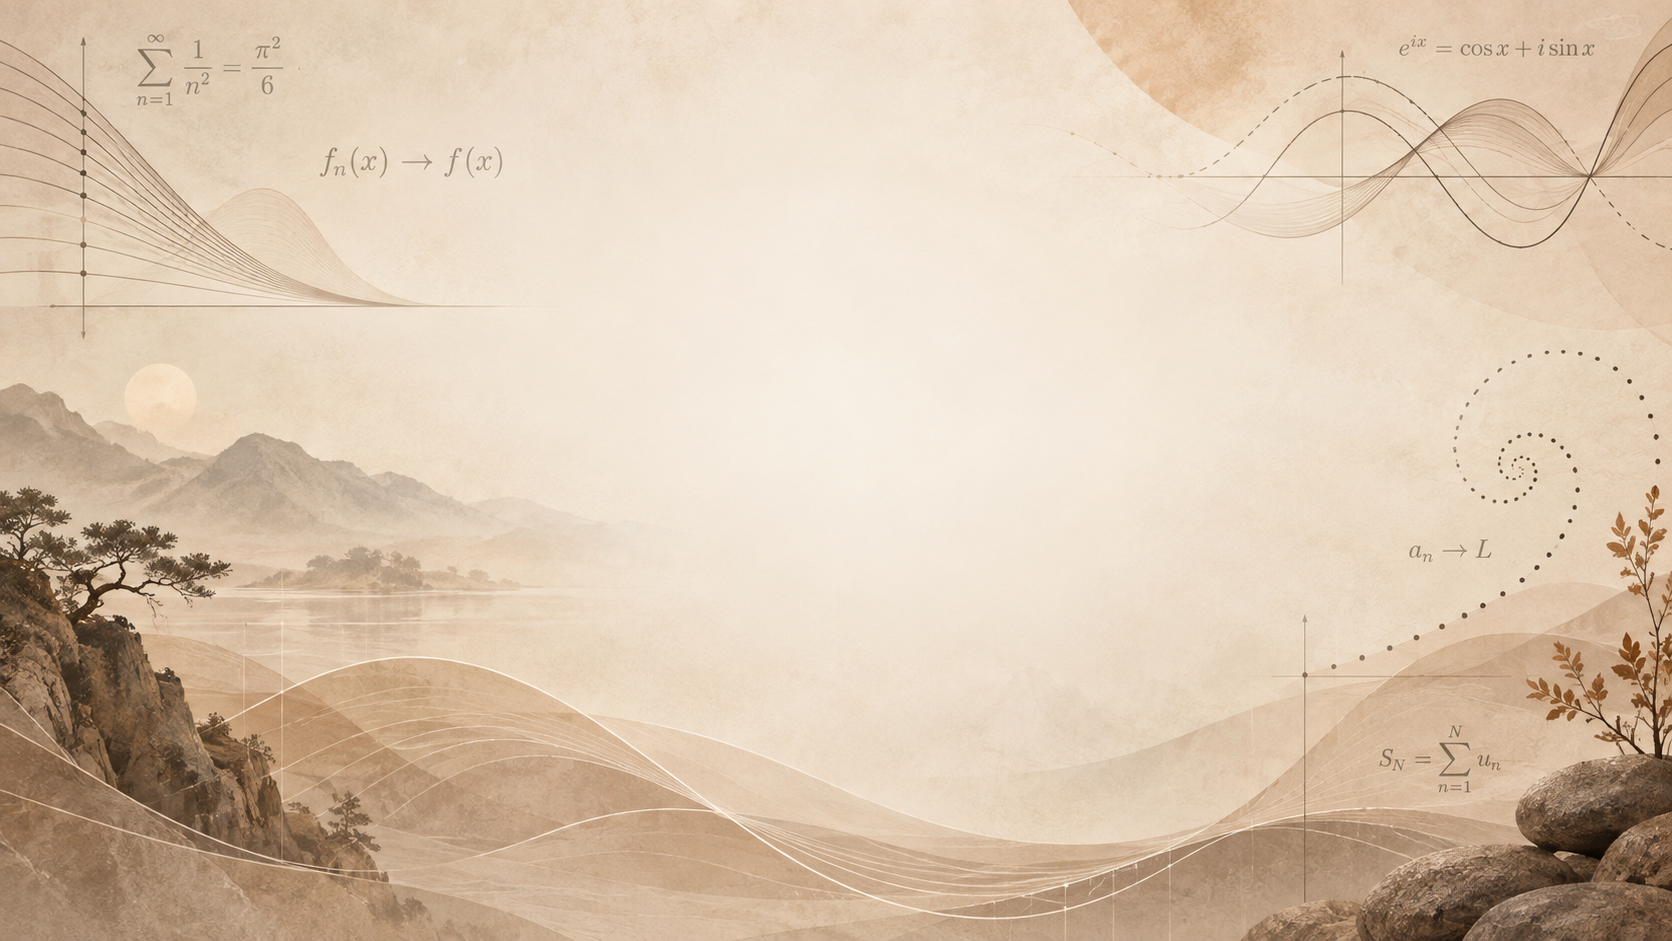
\includegraphics[width=\paperwidth,height=\paperheight,keepaspectratio=false]{chapter_07_bg_00.png}%
}
\begin{frame}[plain]
  \titlepage

  \note{
    Welcome back to Chapter 7, Sequences and Series of Functions. This
    is the third section, Uniform Convergence and Continuity. In the
    previous section we introduced uniform convergence and collected
    tools to verify it. Now we reap the first reward. We will prove
    that uniform convergence allows us to interchange two limit
    processes, and as a consequence, that a uniform limit of continuous
    functions is continuous. We will then see a partial converse, valid
    on compact sets for monotone sequences, and finally we will turn
    the continuous bounded functions on a metric space into a complete
    metric space of their own. Let's begin.
  }
\end{frame}
}

{
\usebackgroundtemplate{%
  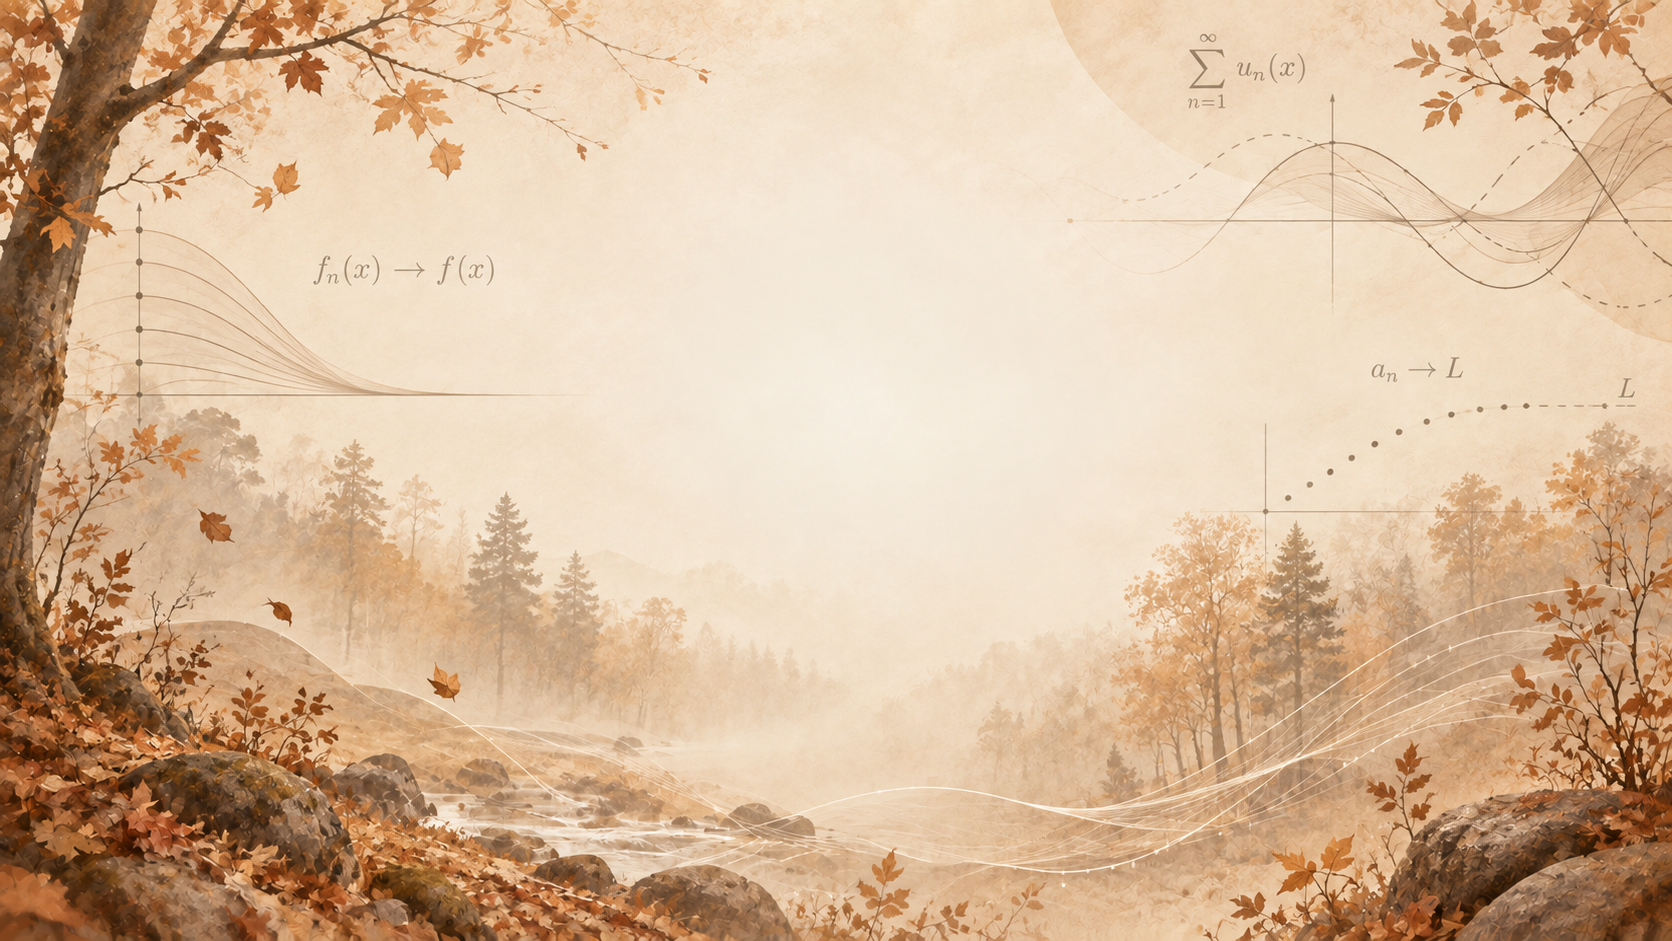
\includegraphics[width=\paperwidth,height=\paperheight,keepaspectratio=false]{chapter_07_bg_01.png}%
}
\begin{frame}[c]{Outline}
  \begin{center}
    \tableofcontents
  \end{center}

  \note{
    Here is the plan. After a short motivation, we prove Theorem 7.11,
    which says that under uniform convergence the limit in "t" and the
    limit in "n" can be interchanged. Then comes Theorem 7.12: uniform
    limits of continuous functions are continuous, together with a
    discussion of why the converse fails. Next is Theorem 7.13, a
    converse for decreasing sequences on compact sets, and an example
    showing that compactness cannot be dropped. Then we introduce the
    space of continuous bounded functions with the supremum norm,
    Definition 7.14, and prove in Theorem 7.15 that it is a complete
    metric space. We close with a summary.
  }
\end{frame}

\section{Motivation}

% --- Build 1/3 ---
\begin{frame}{Why This Section Matters}
  \begin{hlbox}
  \begin{itemize}
    \item The \alert{main problem} of Section 7.1: can limits be interchanged?
      \[
        \lim_{t \to x} \lim_{n \to \infty} f_n(t)
        \;\overset{?}{=}\;
        \lim_{n \to \infty} \lim_{t \to x} f_n(t)
      \]
  \end{itemize}
  \end{hlbox}

  \note{
    Let's recall the main problem of this chapter. In Section 7.1 we
    asked whether properties of the functions "f" sub "n" carry over to
    the limit function. For continuity, the question boils down to the
    identity on the slide. On the left, we first let "n" go to infinity,
    producing the limit function, and then let "t" approach "x". On the
    right, we do it in the opposite order. Continuity of the limit
    function is exactly the statement that these two iterated limits
    agree. So, when can we swap them?
  }
\end{frame}

% --- Build 2/3 ---
\begin{frame}{Why This Section Matters}
  \begin{hlbox}
  \begin{itemize}
    \item The \alert{main problem} of Section 7.1: can limits be interchanged?
      \[
        \lim_{t \to x} \lim_{n \to \infty} f_n(t)
        \;\overset{?}{=}\;
        \lim_{n \to \infty} \lim_{t \to x} f_n(t)
      \]
    \item Under \emph{pointwise} convergence: \alert{no}.\\
      Example 7.3: continuous terms, discontinuous sum
  \end{itemize}
  \end{hlbox}

  \note{
    Under pointwise convergence the answer is no. Recall Example 7.3:
    the series whose terms are "x" squared over 1 plus "x" squared to
    the power "n". Every partial sum is continuous, yet the sum equals
    1 plus "x" squared away from zero and equals zero at the origin, so
    it jumps. The two iterated limits at zero give different answers.
    The trouble was that convergence became slower and slower near the
    bad point.
  }
\end{frame}

% --- Build 3/3 ---
\begin{frame}{Why This Section Matters}
  \begin{hlbox}
  \begin{itemize}
    \item The \alert{main problem} of Section 7.1: can limits be interchanged?
      \[
        \lim_{t \to x} \lim_{n \to \infty} f_n(t)
        \;\overset{?}{=}\;
        \lim_{n \to \infty} \lim_{t \to x} f_n(t)
      \]
    \item Under \emph{pointwise} convergence: \alert{no}.\\
      Example 7.3: continuous terms, discontinuous sum
    \item Under \emph{uniform} convergence (Section 7.2): \alert{yes!}
  \end{itemize}
  \end{hlbox}

  \note{
    In the previous section we introduced uniform convergence precisely
    to rule out this kind of lagging behind. The good news of this
    section is that it works: under uniform convergence, the two limits
    can be interchanged, and continuity is preserved. Let's look at the
    roadmap of the results we will prove.
  }
\end{frame}

\begin{frame}{Roadmap of This Section}
  \vspace{0.4em}
  \begin{center}
  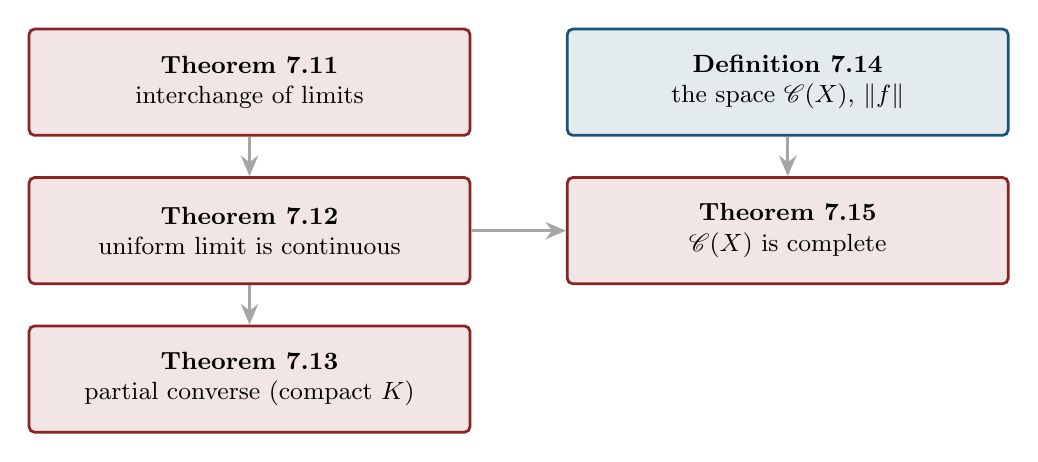
\begin{tikzpicture}[node distance=0.5cm and 1.2cm]
    \node[box=thmcolor] (a) {\textbf{Theorem 7.11}\\ interchange of limits};
    \node[box=thmcolor, below=of a] (b) {\textbf{Theorem 7.12}\\ uniform limit is continuous};
    \node[box=thmcolor, below=of b] (c) {\textbf{Theorem 7.13}\\ partial converse (compact $K$)};
    \node[box=defcolor, right=of a] (d) {\textbf{Definition 7.14}\\ the space $\mathscr{C}(X)$, $\|f\|$};
    \node[box=thmcolor, right=of b] (e) {\textbf{Theorem 7.15}\\ $\mathscr{C}(X)$ is complete};
    \draw[guide, gray!70] (a) -- (b);
    \draw[guide, gray!70] (b) -- (c);
    \draw[guide, gray!70] (d) -- (e);
    \draw[guide, gray!70] (b) -- (e);
  \end{tikzpicture}
  \end{center}

  \note{
    The diagram shows the results of this section. Red boxes are
    theorems, the blue box is a definition. The left column is the main
    line. At the top is Theorem 7.11, the interchange of limits, and the
    gray arrow below it leads to Theorem 7.12, its most important
    consequence: a uniform limit of continuous functions is continuous.
    Another arrow leads down to Theorem 7.13, a partial converse on
    compact sets. In the right column, Definition 7.14 introduces the
    space script capital "C" of capital "X" with its supremum norm. It
    leads down to Theorem 7.15, this space is complete, which also
    relies on Theorem 7.12, as the horizontal arrow shows. Let's start
    with the interchange of limits.
  }
\end{frame}
}

{
\usebackgroundtemplate{%
  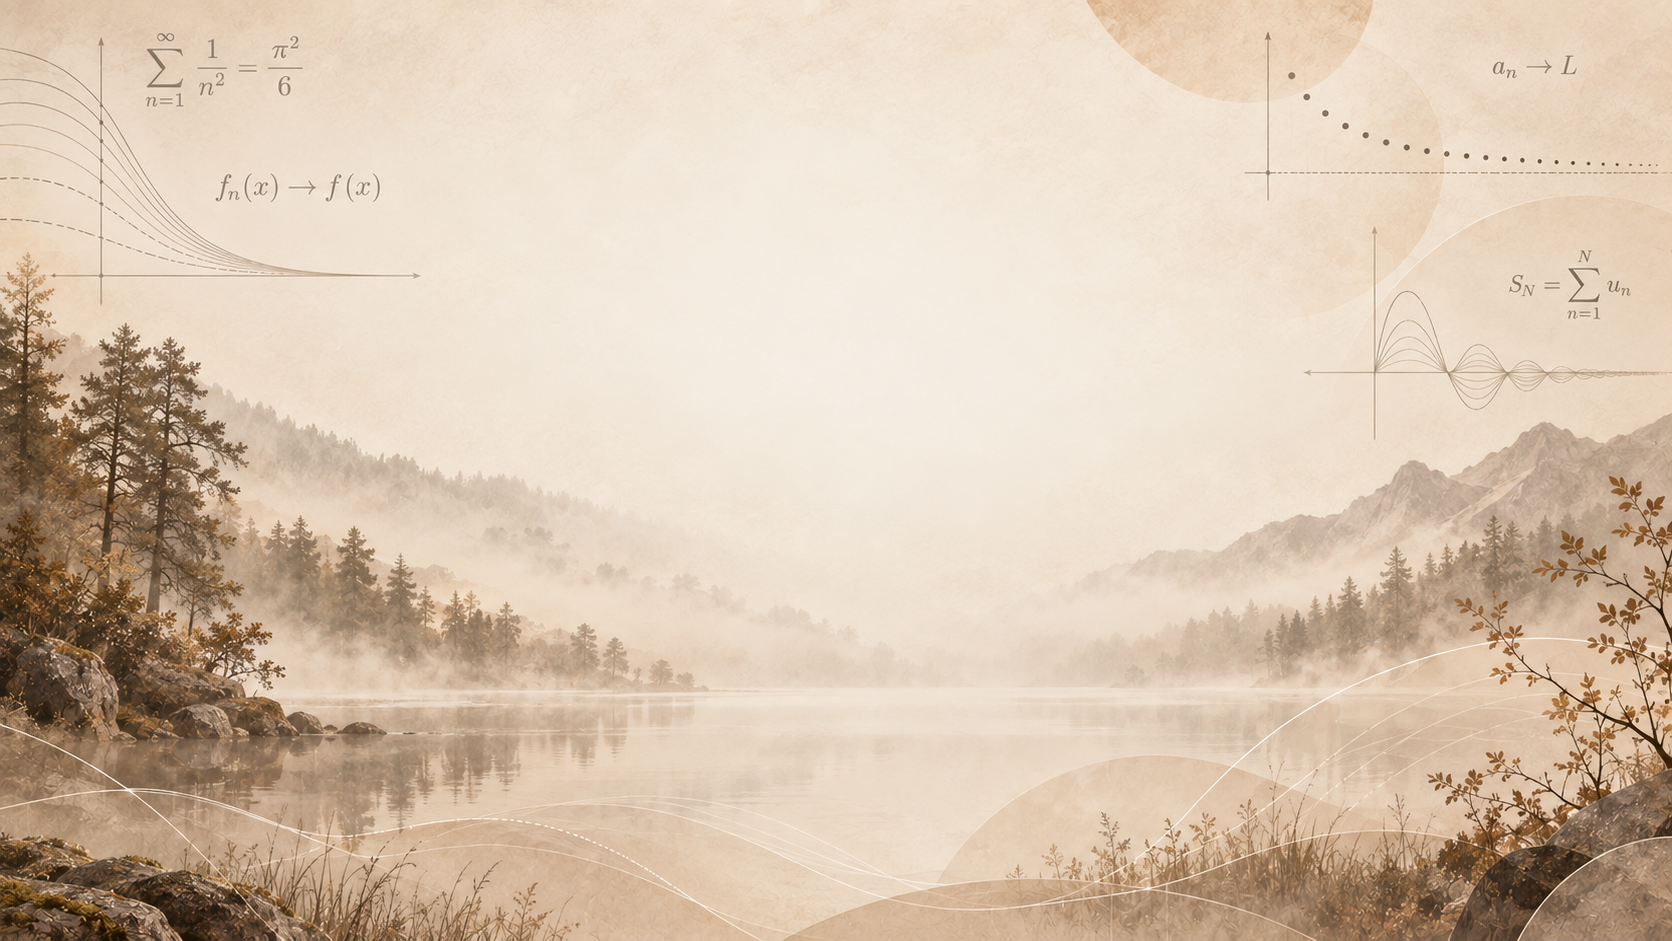
\includegraphics[width=\paperwidth,height=\paperheight,keepaspectratio=false]{chapter_07_bg_02.png}%
}
\section{Interchanging Limits}

% --- Build 1/2 ---
\begin{frame}{Theorem 7.11: Interchange of Limits}
  \begin{thmblock}{Theorem 7.11}
    Suppose $f_n \to f$ \alert{uniformly} on a set $E$ in a metric space. Let $x$
    be a limit point of $E$, and suppose that
    \begin{equation}
      \lim_{t \to x} f_n(t) = A_n \qquad (n = 1, 2, 3, \dots). \tag{15}
    \end{equation}
    Then $\{A_n\}$ converges, and
    \begin{equation}
      \lim_{t \to x} f(t) = \lim_{n \to \infty} A_n. \tag{16}
    \end{equation}
  \end{thmblock}

  \note{
    Here is Theorem 7.11. We have functions "f" sub "n" converging
    uniformly to "f" on a set capital "E" inside a metric space, and a
    limit point "x" of capital "E". The point "x" need not belong to
    capital "E"; we only need to be able to approach it. Assume that
    each "f" sub "n" has a limit as "t" approaches "x", and call it
    capital "A" sub "n"; this is equation 15. The theorem makes two
    claims: first, the numbers capital "A" sub "n" converge; second, "f"
    also has a limit at "x", and it equals the limit of the capital "A"
    sub "n". That is equation 16.
  }
\end{frame}

% --- Build 2/2 ---
\begin{frame}{Theorem 7.11: Interchange of Limits}
  \begin{thmblock}{Theorem 7.11 (in other words)}
    \begin{equation}
      \lim_{t \to x} \lim_{n \to \infty} f_n(t) = \lim_{n \to \infty} \lim_{t \to x} f_n(t). \tag{17}
    \end{equation}
  \end{thmblock}

  \vspace{0.3em}
  \begin{center}
  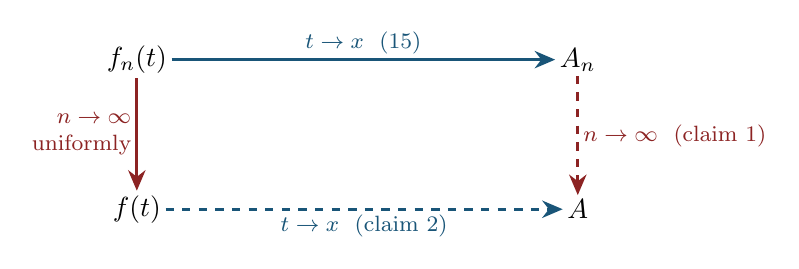
\begin{tikzpicture}[x=1cm,y=1cm, every node/.append style={fill=white, fill opacity=0.65, text opacity=1, inner sep=1.5pt}]
    \node (fn) at (0,1.9) {$f_n(t)$};
    \node (An) at (5.6,1.9) {$A_n$};
    \node (f)  at (0,0) {$f(t)$};
    \node (A)  at (5.6,0) {$A$};
    \draw[guide, defcolor] (fn) -- node[above, font=\footnotesize] {$t \to x$ \ (15)} (An);
    \draw[guide, thmcolor] (fn) -- node[left, font=\footnotesize, align=right] {$n \to \infty$\\ \alert{uniformly}} (f);
    \draw[guide, thmcolor, dashed] (An) -- node[right, font=\footnotesize] {$n \to \infty$ \ (claim 1)} (A);
    \draw[guide, defcolor, dashed] (f) -- node[below, font=\footnotesize] {$t \to x$ \ (claim 2)} (A);
  \end{tikzpicture}
  \end{center}

  \note{
    Rudin summarizes the theorem as equation 17: the iterated limits can
    be interchanged. The square diagram makes this concrete. At the top
    left is "f" sub "n" of "t". The solid blue arrow to the right is
    hypothesis 15: letting "t" approach "x" gives capital "A" sub "n".
    The solid red arrow going down is the uniform convergence to "f" of
    "t". The two dashed arrows are what the theorem delivers: on the
    right, capital "A" sub "n" converges to some number capital "A"; at
    the bottom, "f" of "t" converges to the same capital "A" as "t"
    approaches "x". Both routes around the square end at the same
    corner. Let's see the strategy of the proof.
  }
\end{frame}

\begin{frame}{Proof Strategy: Theorem 7.11}
  \begin{hlbox}
  \textbf{Goal:} Show $A_n \to A$ for some $A$, and then $f(t) \to A$ as $t \to x$.

  \vspace{0.8em}
  \textbf{Approach:}
  \begin{enumerate}
    \item Uniform Cauchy condition for $f_n$ $\Rightarrow$ $\{A_n\}$ is \alert{Cauchy}, so $A_n \to A$.
    \item Split $|f(t) - A|$ into \alert{three} pieces by the triangle inequality.
    \item Pick one good $n$: makes two pieces $\leq \varepsilon/3$.
    \item For \emph{that} $n$, choose $t$ close to $x$: third piece $\leq \varepsilon/3$.
  \end{enumerate}

  \vspace{0.5em}
  \textbf{Technique:} the $\varepsilon/3$ argument.
  \end{hlbox}

  \note{
    Before the details, here is the plan. The goal has two parts: find
    the limit capital "A" of the numbers capital "A" sub "n", and then
    show that "f" of "t" tends to capital "A". Step 1 uses the Cauchy
    criterion for uniform convergence to show that the capital "A" sub
    "n" form a Cauchy sequence. Step 2 splits the distance from "f" of
    "t" to capital "A" into three pieces. In step 3 we fix a single good
    index "n" that controls two of the pieces, and in step 4 we use
    hypothesis 15 for that one index to control the third piece. This
    is the classical epsilon over 3 argument, which we will meet again
    and again in this chapter.
  }
\end{frame}

% --- Build 1/2 ---
\begin{frame}{Proof of Theorem 7.11 --- Step 1: $\{A_n\}$ Converges}
  \begin{proofblock}{Step 1: $\{A_n\}$ is a Cauchy sequence}
    Let $\varepsilon > 0$. By uniform convergence (Theorem 7.8), there is $N$ such that
    $n \geq N$, $m \geq N$, $t \in E$ imply
    \begin{equation}
      |f_n(t) - f_m(t)| \leq \varepsilon. \tag{18}
    \end{equation}
  \end{proofblock}

  \note{
    Let's begin. Fix epsilon greater than zero. Since the convergence is
    uniform, the Cauchy criterion, Theorem 7.8, gives a threshold capital
    "N" such that inequality 18 holds for all indices "n" and "m" at
    least capital "N". The key phrase is "t" in capital "E": the
    inequality holds for every point "t" simultaneously, with the same
    capital "N". This is exactly what will let us move "t" toward "x"
    while keeping the indices fixed.
  }
\end{frame}

% --- Build 2/2 ---
\begin{frame}{Proof of Theorem 7.11 --- Step 1: $\{A_n\}$ Converges}
  \begin{proofblock}{Step 1: $\{A_n\}$ is a Cauchy sequence}
    Let $\varepsilon > 0$. By uniform convergence (Theorem 7.8), there is $N$ such that
    $n \geq N$, $m \geq N$, $t \in E$ imply
    \begin{equation}
      |f_n(t) - f_m(t)| \leq \varepsilon. \tag{18}
    \end{equation}
    Letting $t \to x$ in (18):
    \[
      |A_n - A_m| \leq \varepsilon \qquad (n, m \geq N).
    \]
    So $\{A_n\}$ is \alert{Cauchy}, hence converges (Theorem 3.11), say to $A$.
  \end{proofblock}

  \note{
    Now keep "n" and "m" fixed and let "t" approach "x" in inequality
    18. By hypothesis 15, "f" sub "n" of "t" tends to capital "A" sub
    "n" and "f" sub "m" of "t" tends to capital "A" sub "m", and since
    non strict inequalities survive limits, capital "A" sub "n" and
    capital "A" sub "m" differ by at most epsilon. So the capital "A"
    sub "n" form a Cauchy sequence of complex numbers, which converges
    by Theorem 3.11. Call its limit capital "A". That settles the first
    claim of the theorem.
  }
\end{frame}

% --- Build 1/2 ---
\begin{frame}{Proof of Theorem 7.11 --- Step 2: Three Pieces}
  \begin{proofblock}{Step 2: Triangle inequality}
    \begin{equation}
      |f(t) - A| \leq \underbrace{|f(t) - f_n(t)|}_{\text{uniform conv.}}
        + \underbrace{|f_n(t) - A_n|}_{t \text{ near } x}
        + \underbrace{|A_n - A|}_{A_n \to A}. \tag{19}
    \end{equation}
  \end{proofblock}

  \note{
    Now we want to show that "f" of "t" is close to capital "A" when "t"
    is close to "x". Inequality 19 inserts two intermediate points,
    "f" sub "n" of "t" and capital "A" sub "n", and applies the triangle
    inequality. Each of the three pieces is controlled by a different
    fact, as the labels under the braces indicate. The first piece is
    small by uniform convergence. The second is small when "t" is near
    "x", by hypothesis 15. The third is small because capital "A" sub
    "n" converges to capital "A", as shown in step 1. Let's see a
    picture of this chain.
  }
\end{frame}

% --- Build 2/2 ---
\begin{frame}{Proof of Theorem 7.11 --- Step 2: Three Pieces}
  \begin{proofblock}{Step 2: Triangle inequality}
    \begin{equation}
      |f(t) - A| \leq \underbrace{|f(t) - f_n(t)|}_{\text{uniform conv.}}
        + \underbrace{|f_n(t) - A_n|}_{t \text{ near } x}
        + \underbrace{|A_n - A|}_{A_n \to A}. \tag{19}
    \end{equation}
  \end{proofblock}

  \vspace{0.2em}
  \begin{center}
  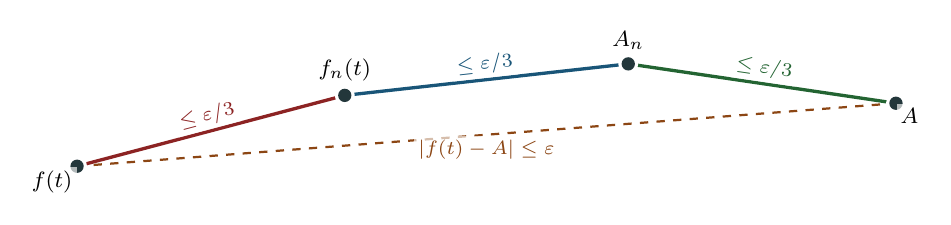
\begin{tikzpicture}[x=1cm,y=1cm, every node/.append style={fill=white, fill opacity=0.65, text opacity=1, inner sep=1.5pt}]
    \coordinate (P0) at (0,0);
    \coordinate (P1) at (3.4,0.9);
    \coordinate (P2) at (7.0,1.3);
    \coordinate (P3) at (10.4,0.8);
    \draw[thmcolor, line width=1.2pt] (P0) -- node[above, sloped, font=\scriptsize] {$\leq \varepsilon/3$} (P1);
    \draw[defcolor, line width=1.2pt] (P1) -- node[above, sloped, font=\scriptsize] {$\leq \varepsilon/3$} (P2);
    \draw[proofcolor, line width=1.2pt] (P2) -- node[above, sloped, font=\scriptsize] {$\leq \varepsilon/3$} (P3);
    \draw[mAccent, line width=0.8pt, dashed] (P0) -- node[below, font=\scriptsize] {$|f(t) - A| \leq \varepsilon$} (P3);
    \dotpt{mDarkTeal}{(P0)} \node[below left, font=\footnotesize] at (P0) {$f(t)$};
    \dotpt{mDarkTeal}{(P1)} \node[above, font=\footnotesize] at ($(P1)+(0,0.12)$) {$f_n(t)$};
    \dotpt{mDarkTeal}{(P2)} \node[above, font=\footnotesize] at ($(P2)+(0,0.12)$) {$A_n$};
    \dotpt{mDarkTeal}{(P3)} \node[below right, font=\footnotesize] at (P3) {$A$};
  \end{tikzpicture}
  \end{center}

  \note{
    The picture shows the chain as a path of three hops in the complex
    plane. We start at "f" of "t" on the left. The red hop goes to "f"
    sub "n" of "t", the blue hop continues to capital "A" sub "n", and
    the green hop ends at capital "A" on the right. If each hop has
    length at most epsilon over 3, then the direct dashed orange
    shortcut from "f" of "t" to capital "A" has length at most epsilon.
    The subtle point is the order in which we make the choices, which is
    the content of the next step.
  }
\end{frame}

% --- Build 1/2 ---
\begin{frame}{Proof of Theorem 7.11 --- Steps 3--4: Choose $n$, Then $t$}
  \begin{proofblock}{Step 3: Fix one good $n$}
    Choose $n$ such that
    \begin{align}
      |f(t) - f_n(t)| &\leq \tfrac{\varepsilon}{3} \quad \text{for all } t \in E
        \quad (\text{uniform conv.}), \tag{20}\\
      |A_n - A| &\leq \tfrac{\varepsilon}{3}. \tag{21}
    \end{align}
  \end{proofblock}

  \note{
    Now the order of choices. First we choose the index "n". Uniform
    convergence lets us pick "n" so large that inequality 20 holds for
    every "t" in capital "E" at once, and since capital "A" sub "n"
    converges to capital "A", we can also make inequality 21 hold. This
    takes care of the red hop and the green hop in our picture. From
    now on, "n" is frozen.
  }
\end{frame}

% --- Build 2/2 ---
\begin{frame}{Proof of Theorem 7.11 --- Steps 3--4: Choose $n$, Then $t$}
  \begin{proofblock}{Step 3: Fix one good $n$}
    Choose $n$ such that
    \begin{align}
      |f(t) - f_n(t)| &\leq \tfrac{\varepsilon}{3} \quad \text{for all } t \in E
        \quad (\text{uniform conv.}), \tag{20}\\
      |A_n - A| &\leq \tfrac{\varepsilon}{3}. \tag{21}
    \end{align}
  \end{proofblock}
  \begin{proofblock}{Step 4: Then choose $t$ near $x$}
    For \alert{this} $n$, by (15) pick a neighborhood $V$ of $x$ with
    \begin{equation}
      |f_n(t) - A_n| \leq \tfrac{\varepsilon}{3} \qquad (t \in V \cap E,\ t \neq x). \tag{22}
    \end{equation}
  \end{proofblock}


  \note{
    Only now, with "n" frozen, do we look at "t". Hypothesis 15 for this
    single function gives a neighborhood capital "V" of "x" in which "f"
    sub "n" of "t" is within epsilon over 3 of capital "A" sub "n"; that
    is inequality 22, the blue hop. Notice why uniformity is essential:
    inequality 20 must hold at every "t" in capital "V", a neighborhood
    we did not know when we chose "n". With merely pointwise
    convergence, the index needed at "t" could grow without bound as
    "t" approaches "x".
  }
\end{frame}

\begin{frame}{Proof of Theorem 7.11 --- Conclusion}
  \begin{proofblock}{Conclusion}
    Substituting (20)--(22) into (19):
    \[
      |f(t) - A| \leq \tfrac{\varepsilon}{3} + \tfrac{\varepsilon}{3} + \tfrac{\varepsilon}{3}
      = \varepsilon \qquad (t \in V \cap E,\ t \neq x).
    \]
    Hence $\displaystyle \boxed{\lim_{t \to x} f(t) = A = \lim_{n \to \infty} A_n}$,
    which is (16). \hfill $\blacksquare$
  \end{proofblock}

  \vspace{0.3em}
  \hl{\textbf{Key idea:} uniformity lets us fix $n$ \alert{before} choosing $t$.}

  \note{
    Putting the three estimates 20, 21, and 22 into inequality 19, each
    piece contributes at most epsilon over 3, so "f" of "t" is within
    epsilon of capital "A" for every "t" in the neighborhood capital "V"
    other than "x" itself. Since epsilon was arbitrary, "f" of "t"
    tends to capital "A" as "t" approaches "x", which is equation 16,
    and the proof is complete. The line below the box captures the heart
    of the argument: uniformity lets us fix the index "n" before choosing
    the point "t". Next, the most important consequence.
  }
\end{frame}
}

{
\usebackgroundtemplate{%
  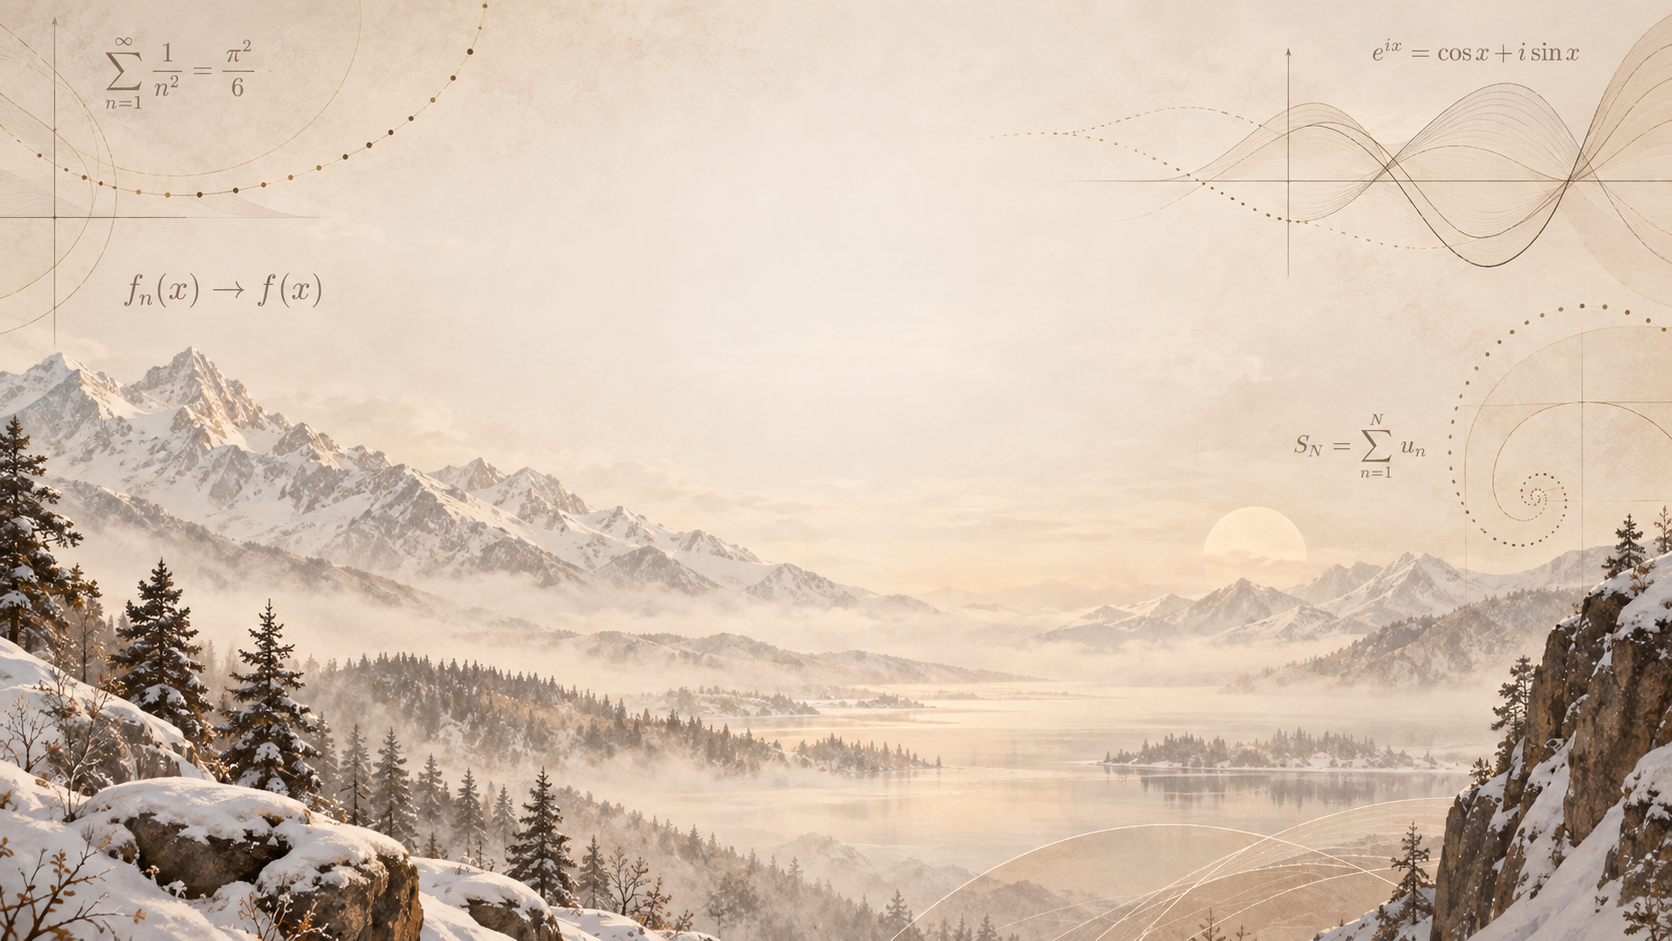
\includegraphics[width=\paperwidth,height=\paperheight,keepaspectratio=false]{chapter_07_bg_03.png}%
}
\section{Continuity of Uniform Limits}

% --- Build 1/2 ---
\begin{frame}{Theorem 7.12: Uniform Limits Are Continuous}
  \begin{thmblock}{Theorem 7.12}
    If $\{f_n\}$ is a sequence of \alert{continuous} functions on $E$, and if
    $f_n \to f$ \alert{uniformly} on $E$, then $f$ is \alert{continuous} on $E$.
  \end{thmblock}

  \note{
    Here is Theorem 7.12, which Rudin calls a very important result. If
    each "f" sub "n" is continuous on capital "E" and the convergence is
    uniform, then the limit "f" is continuous. In the language of the
    main problem: continuity survives uniform limits. This is exactly
    what failed in Example 7.3, where the convergence was only
    pointwise. Rudin notes that it is an immediate corollary of the
    previous theorem; let's see why.
  }
\end{frame}

% --- Build 2/2 ---
\begin{frame}{Theorem 7.12: Uniform Limits Are Continuous}
  \begin{thmblock}{Theorem 7.12}
    If $\{f_n\}$ is a sequence of \alert{continuous} functions on $E$, and if
    $f_n \to f$ \alert{uniformly} on $E$, then $f$ is \alert{continuous} on $E$.
  \end{thmblock}

  \vspace{0.3em}
  \begin{proofblock}{Proof (immediate from Theorem 7.11)}
    Let $x \in E$. If $x$ is isolated, $f$ is continuous at $x$ trivially. Otherwise
    $x$ is a limit point, and $A_n = \lim_{t \to x} f_n(t) = f_n(x)$, so by (16)
    \[
      \lim_{t \to x} f(t) = \lim_{n \to \infty} f_n(x) = f(x). \qquad \blacksquare
    \]
  \end{proofblock}

  \note{
    The green box gives the proof. Take a point "x" of capital "E". At an
    isolated point every function is continuous, so there is nothing to
    prove. Otherwise "x" is a limit point, and since "f" sub "n" is
    continuous, the limit capital "A" sub "n" is just "f" sub "n" of
    "x". Equation 16 then says the limit of "f" of "t" as "t" approaches
    "x" equals the limit of "f" sub "n" of "x", which is "f" of "x" by
    pointwise convergence. That is continuity at "x". Next, a practical
    use of this theorem.
  }
\end{frame}

% --- Build 1/2 ---
\begin{frame}{Using Theorem 7.12 as a Test}
  \begin{hlbox}
  \textbf{Contrapositive:} continuous $f_n \to f$, but $f$ \alert{discontinuous}
  $\;\Longrightarrow\;$ convergence is \alert{not uniform}.
  \end{hlbox}

  \vspace{0.2em}
  \begin{columns}[T]
    \begin{column}{0.44\textwidth}
      \begin{exblock}{Example: $f_n(x) = x^n$ on $[0,1]$}
        \[
          f(x) = \begin{cases} 0 & 0 \leq x < 1,\\ 1 & x = 1. \end{cases}
        \]
        Jump at $x = 1$ $\Rightarrow$ not uniform.
      \end{exblock}
    \end{column}
    \begin{column}{0.54\textwidth}
      \begin{center}
      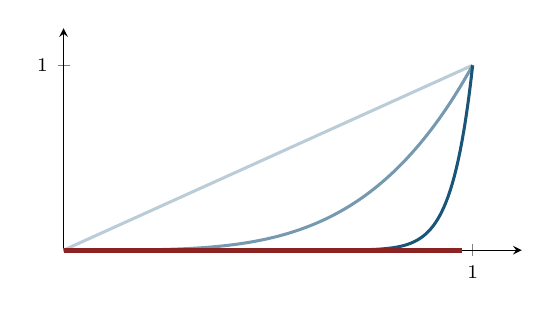
\begin{tikzpicture}
        \begin{axis}[
          width=7.4cm, height=4.4cm,
          axis lines=left,
          xmin=0, xmax=1.12, ymin=0, ymax=1.2,
          xtick={1}, ytick={1},
          tick label style={font=\scriptsize},
          clip=false,
        ]
          \addplot[defcolor!30, line width=1.1pt, domain=0:1, samples=60] {x};
          \addplot[defcolor!60, line width=1.1pt, domain=0:1, samples=100] {x^4};
          \addplot[defcolor, line width=1.1pt, domain=0:1, samples=200] {x^20};
          \addplot[thmcolor, line width=1.8pt, domain=0:0.975, samples=2] {0};
        \end{axis}
      \end{tikzpicture}
      \end{center}
    \end{column}
  \end{columns}

  \note{
    Theorem 7.12 gives a quick test for non uniform convergence, stated
    at the top as the contrapositive: if continuous functions converge
    to a discontinuous limit, the convergence cannot be uniform. The
    orange box on the left recalls the test case from the previous
    section: the powers of "x" on the unit interval converge to the
    function that is zero on the half open interval and one at the
    point 1. In the plot, the three blue curves, from light to dark, are
    "x", "x" to the fourth, and "x" to the twentieth, and the thick red
    segment along the bottom is the limit function away from 1.
  }
\end{frame}

% --- Build 2/2 ---
\begin{frame}{Using Theorem 7.12 as a Test}
  \begin{hlbox}
  \textbf{Contrapositive:} continuous $f_n \to f$, but $f$ \alert{discontinuous}
  $\;\Longrightarrow\;$ convergence is \alert{not uniform}.
  \end{hlbox}

  \vspace{0.2em}
  \begin{columns}[T]
    \begin{column}{0.44\textwidth}
      \begin{exblock}{Example: $f_n(x) = x^n$ on $[0,1]$}
        \[
          f(x) = \begin{cases} 0 & 0 \leq x < 1,\\ 1 & x = 1. \end{cases}
        \]
        Jump at $x = 1$ $\Rightarrow$ not uniform.
      \end{exblock}
      \vspace{0.2em}
      \hl{Same for Example 7.3 (jump at $0$).}
    \end{column}
    \begin{column}{0.54\textwidth}
      \begin{center}
      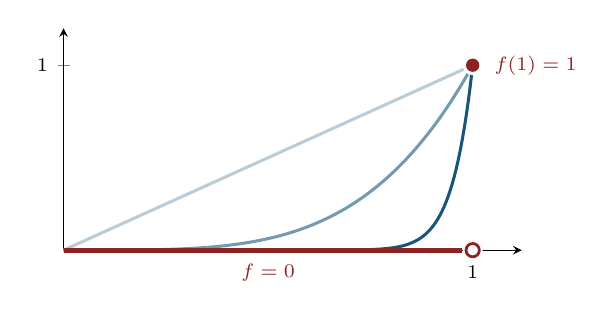
\begin{tikzpicture}
        \begin{axis}[
          width=7.4cm, height=4.4cm,
          axis lines=left,
          xmin=0, xmax=1.12, ymin=0, ymax=1.2,
          xtick={1}, ytick={1},
          tick label style={font=\scriptsize},
          clip=false,
        ]
          \addplot[defcolor!30, line width=1.1pt, domain=0:1, samples=60] {x};
          \addplot[defcolor!60, line width=1.1pt, domain=0:1, samples=100] {x^4};
          \addplot[defcolor, line width=1.1pt, domain=0:1, samples=200] {x^20};
          \addplot[thmcolor, line width=1.8pt, domain=0:0.975, samples=2] {0};
          \opendotpt{thmcolor}{(axis cs:1,0)}
          \dotpt{thmcolor}{(axis cs:1,1)}
          \node[thmcolor, font=\scriptsize, anchor=west] at (axis cs:1.03,1) {$f(1) = 1$};
          \node[thmcolor, font=\scriptsize, anchor=north] at (axis cs:0.5,-0.02) {$f = 0$};
        \end{axis}
      \end{tikzpicture}
      \end{center}
    \end{column}
  \end{columns}

  \note{
    Now look at the point 1 in the plot. The red open circle at height
    zero marks where the limit function would continue, but the solid
    red dot at height one, labeled "f" of 1 equals 1, shows the actual
    value there. That jump is a discontinuity, so by Theorem 7.12 the
    convergence cannot be uniform, confirming what we computed directly
    last time. The line under the orange box notes that the same
    reasoning disposes of Example 7.3: every partial sum of that series
    is continuous, but the sum jumps at the origin, so the series does
    not converge uniformly on any interval containing zero. Next, what
    about the converse?
  }
\end{frame}

% --- Build 1/2 ---
\begin{frame}{The Converse of Theorem 7.12 Fails}
  \begin{exblock}{Example 7.6 revisited}
    $f_n(x) = n^2 x (1 - x^2)^n$ on $[0,1]$: each $f_n$ continuous,
    $f_n \to f = 0$ pointwise, and $f$ is \alert{continuous}.
  \end{exblock}

  \note{
    Is the converse of Theorem 7.12 true? That is, if continuous
    functions converge pointwise to a continuous limit, must the
    convergence be uniform? The answer is no, and Rudin points to
    Example 7.6 from the first section. There, "f" sub "n" of "x" is "n"
    squared times "x" times 1 minus "x" squared to the power "n", on the
    unit interval. Each "f" sub "n" is a polynomial, hence continuous.
    At every point the values tend to zero, so the limit function is the
    zero function, which is certainly continuous.
  }
\end{frame}

% --- Build 2/2 ---
\begin{frame}{The Converse of Theorem 7.12 Fails}
  \begin{exblock}{Example 7.6 revisited}
    $f_n(x) = n^2 x (1 - x^2)^n$ on $[0,1]$: each $f_n$ continuous,
    $f_n \to f = 0$ pointwise, and $f$ is \alert{continuous}.
  \end{exblock}

  \begin{columns}[T]
    \begin{column}{0.46\textwidth}
      \begin{hlbox}
      But (Theorem 7.9):
      \[
        M_n = \sup_{[0,1]} |f_n| \geq f_n\!\left(\tfrac{1}{\sqrt{n}}\right) \to \infty.
      \]
      \alert{Not uniform!}
      \end{hlbox}
    \end{column}
    \begin{column}{0.52\textwidth}
      \begin{center}
      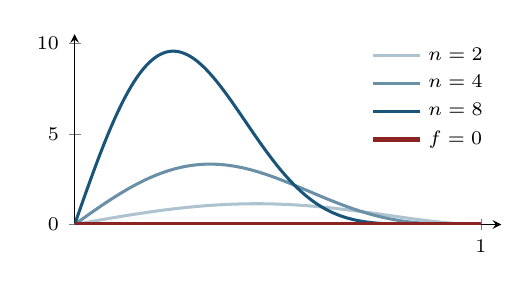
\begin{tikzpicture}
        \begin{axis}[
          width=7.0cm, height=4.0cm,
          axis lines=left,
          xmin=0, xmax=1.05, ymin=0, ymax=10.5,
          xtick={1}, ytick={0,5,10},
          tick label style={font=\scriptsize},
          legend style={font=\scriptsize, at={(0.99,0.99)}, anchor=north east,
            draw=none, fill=white, fill opacity=0.8, text opacity=1},
        ]
          \addplot[defcolor!35, line width=1.1pt, domain=0:1, samples=120] {4*x*(1-x^2)^2};
          \addlegendentry{$n = 2$}
          \addplot[defcolor!65, line width=1.1pt, domain=0:1, samples=160] {16*x*(1-x^2)^4};
          \addlegendentry{$n = 4$}
          \addplot[defcolor, line width=1.1pt, domain=0:1, samples=250] {64*x*(1-x^2)^8};
          \addlegendentry{$n = 8$}
          \addplot[thmcolor, line width=1.8pt, domain=0:1, samples=2] {0};
          \addlegendentry{$f = 0$}
        \end{axis}
      \end{tikzpicture}
      \end{center}
    \end{column}
  \end{columns}

  \note{
    Yet the convergence is not uniform. Apply Theorem 7.9 from the
    previous section: the worst case error capital "M" sub "n" is at
    least the value of "f" sub "n" at 1 over the square root of "n",
    which equals "n" to the three halves times 1 minus 1 over "n", to
    the power "n", roughly "n" to the three halves over "e". This tends
    to infinity, not to zero. The plot shows the bumps for "n" equal to
    2, 4, and 8, in increasingly dark blue: they get taller and move
    toward the origin, while the red limit function stays flat at zero.
    So a continuous limit does not force uniform convergence. But there
    is one situation where it does, and that is our next theorem.
  }
\end{frame}
}

{
\usebackgroundtemplate{%
  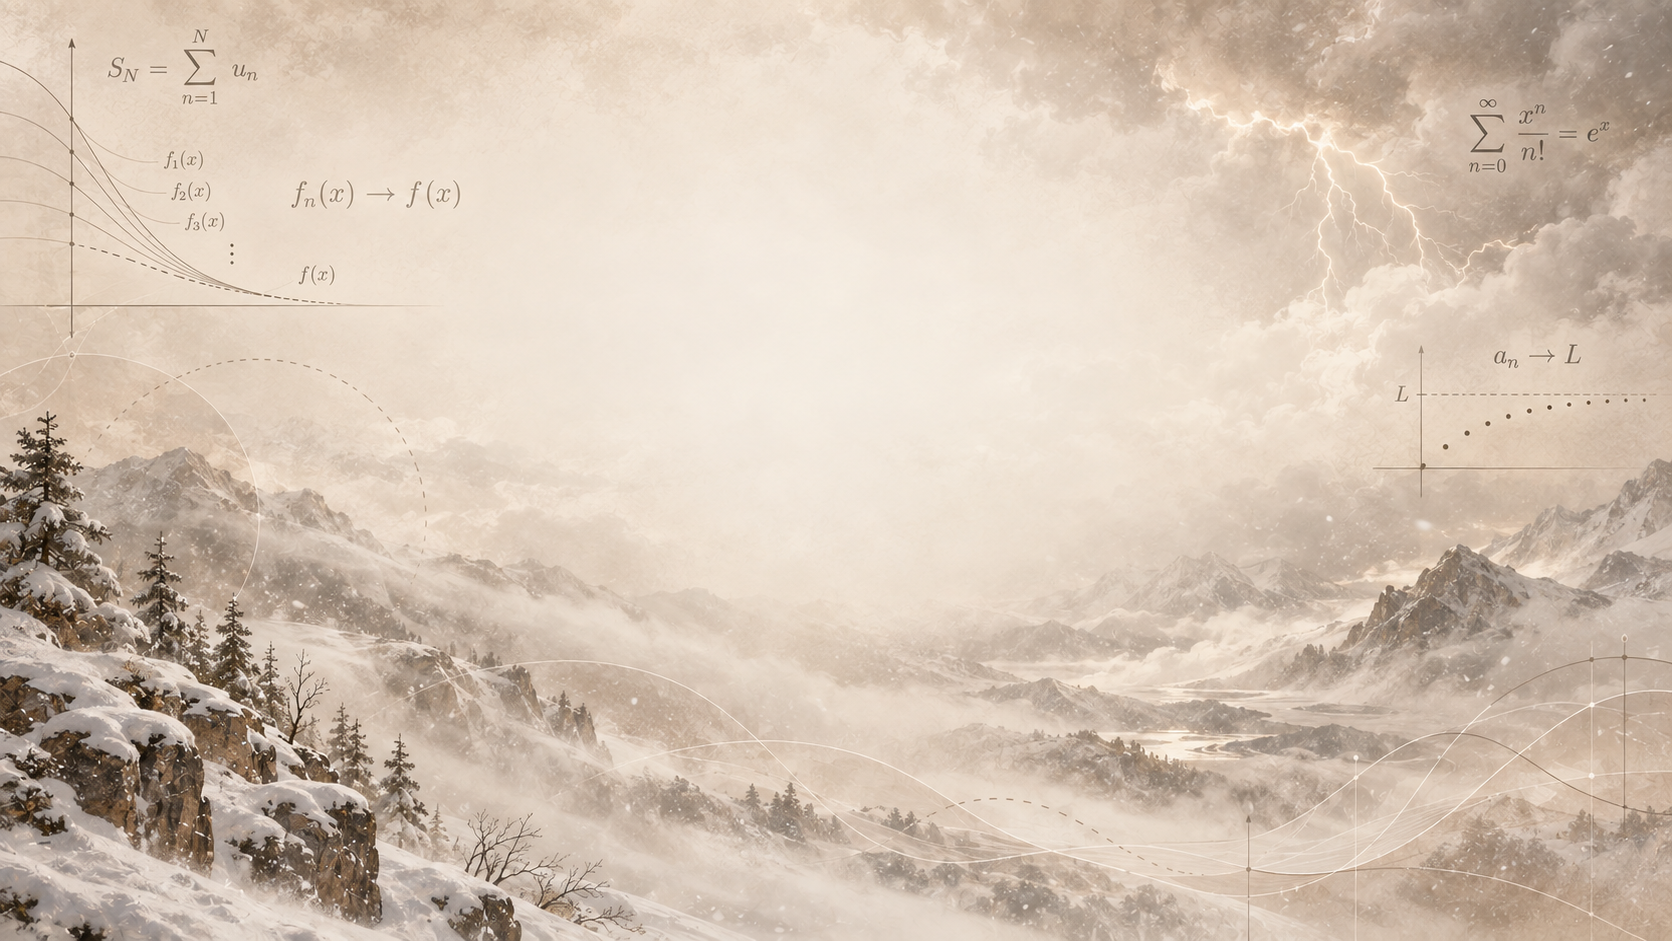
\includegraphics[width=\paperwidth,height=\paperheight,keepaspectratio=false]{chapter_07_bg_04.png}%
}
\section{Monotone Convergence on Compact Sets}

% --- Build 1/2 ---
\begin{frame}{Theorem 7.13: A Partial Converse}
  \begin{thmblock}{Theorem 7.13}
    Suppose $K$ is \alert{compact}, and
    \begin{enumerate}
      \item[(a)] $\{f_n\}$ is a sequence of continuous functions on $K$,
      \item[(b)] $\{f_n\}$ converges pointwise to a \alert{continuous} function $f$ on $K$,
      \item[(c)] $f_n(x) \geq f_{n+1}(x)$ for all $x \in K$, $n = 1, 2, 3, \dots$ \ (\alert{monotone}).
    \end{enumerate}
    Then $f_n \to f$ \alert{uniformly} on $K$.
  \end{thmblock}

  \vspace{0.2em}
  \hl{\textit{(Known as \textbf{Dini's theorem}.)}}

  \note{
    Here is Theorem 7.13, often called Dini's theorem, although Rudin
    does not name it. Let capital "K" be a compact set, and assume
    three things. Condition "a": each "f" sub "n" is continuous.
    Condition "b": the sequence converges pointwise to a limit "f" that
    is itself continuous. Condition "c": the sequence is monotonically
    decreasing at every point. Then the conclusion is that the
    convergence is uniform. So on a compact set, continuity of the
    limit plus monotonicity is enough to upgrade pointwise convergence
    to uniform convergence. Note that the values "f" sub "n" are real
    here, since we compare them. Let's picture the hypotheses.
  }
\end{frame}

% --- Build 2/2 ---
\begin{frame}{Theorem 7.13: A Partial Converse}
  \begin{columns}[T]
    \begin{column}{0.40\textwidth}
      \vspace{0.8em}
      \begin{hlbox}
      \begin{itemize}
        \item $K = [0,1]$ (compact)
        \item $f_n = f + g_n$ with\\
          $g_n(x) = 4x^n(1 - x)$
        \item $f_n$ \alert{decrease} to $f$ at every point
      \end{itemize}
      \end{hlbox}
    \end{column}
    \begin{column}{0.58\textwidth}
      \begin{center}
      \begin{tikzpicture}
        \begin{axis}[
          width=8.0cm, height=5.8cm,
          axis lines=left,
          xmin=0, xmax=1.05, ymin=0, ymax=2.0,
          xtick={0,1}, ytick=\empty,
          tick label style={font=\scriptsize},
          legend style={font=\scriptsize, at={(0.01,0.99)}, anchor=north west,
            draw=none, fill=white, fill opacity=0.8, text opacity=1},
        ]
          \addplot[defcolor!30, line width=1.1pt, domain=0:1, samples=120]
            {0.5 + 0.2*sin(deg(5*x)) + dinig(x,1)};
          \addlegendentry{$f_1$}
          \addplot[defcolor!55, line width=1.1pt, domain=0:1, samples=120]
            {0.5 + 0.2*sin(deg(5*x)) + dinig(x,2)};
          \addlegendentry{$f_2$}
          \addplot[defcolor!80, line width=1.1pt, domain=0:1, samples=150]
            {0.5 + 0.2*sin(deg(5*x)) + dinig(x,4)};
          \addlegendentry{$f_4$}
          \addplot[defcolor, line width=1.1pt, domain=0:1, samples=200]
            {0.5 + 0.2*sin(deg(5*x)) + dinig(x,8)};
          \addlegendentry{$f_8$}
          \addplot[thmcolor, line width=1.8pt, domain=0:1, samples=120]
            {0.5 + 0.2*sin(deg(5*x))};
          \addlegendentry{$f$}
        \end{axis}
      \end{tikzpicture}
      \end{center}
    \end{column}
  \end{columns}

  \note{
    Here is an illustration. The compact set is the unit interval. The
    thick red curve is a continuous limit function "f". On top of it we
    add bumps "g" sub "n" of "x" equal to 4 times "x" to the "n" times 1
    minus "x"; these are continuous, nonnegative, and decrease in "n" at
    every point. The blue curves, from light to dark, are "f" sub 1,
    "f" sub 2, "f" sub 4, and "f" sub 8. Each lies below the previous
    one, and they settle down onto the red curve. Theorem 7.13 promises
    that the settling happens uniformly over the whole interval. Let's
    see how compactness enters the proof.
  }
\end{frame}

\begin{frame}{Proof Strategy: Theorem 7.13}
  \begin{hlbox}
  \textbf{Goal:} $g_n = f_n - f \to 0$ uniformly on $K$.

  \vspace{0.8em}
  \textbf{Approach:}
  \begin{enumerate}
    \item Reduce to $g_n \geq 0$, continuous, decreasing, $g_n \to 0$ pointwise.
    \item Consider the ``bad sets'' $K_n = \{x \in K : g_n(x) \geq \varepsilon\}$.
    \item They are \alert{compact} and \alert{nested}, with empty intersection.
    \item Compactness $\Rightarrow$ some $K_N$ is \alert{empty} $\Rightarrow$ $g_n < \varepsilon$ for $n \geq N$.
  \end{enumerate}

  \vspace{0.5em}
  \textbf{Technique:} nested compact sets (Theorem 2.36).
  \end{hlbox}

  \note{
    Here is the plan. First we subtract the limit, reducing to a
    sequence "g" sub "n" that decreases to zero. Then, for a given
    epsilon, we look at the bad set capital "K" sub "n": the points
    where "g" sub "n" is still at least epsilon. These bad sets are
    compact and nested, and pointwise convergence says no point stays
    bad forever, so their intersection is empty. Finally, a
    compactness property from Chapter 2, Theorem 2.36, forces one of
    the bad sets to be empty already. From then on "g" sub "n" is less
    than epsilon everywhere, which is uniform convergence.
  }
\end{frame}

\begin{frame}{Proof of Theorem 7.13 --- Step 1: Reduction}
  \begin{proofblock}{Step 1: Put $g_n = f_n - f$}
    \begin{itemize}
      \item $g_n$ is \alert{continuous} (by (a) and (b))
      \item $g_n \to 0$ \alert{pointwise} (by (b))
      \item $g_n \geq g_{n+1}$ (by (c)), hence $g_n \geq 0$
    \end{itemize}
    \textbf{To prove:} $g_n \to 0$ \alert{uniformly} on $K$.
  \end{proofblock}

  \note{
    We begin by subtracting the limit. Put "g" sub "n" equal to "f" sub
    "n" minus "f". Since both "f" sub "n" and "f" are continuous, so is
    "g" sub "n". Pointwise convergence of "f" sub "n" to "f" means "g"
    sub "n" tends to zero at each point. And the monotonicity in
    condition "c" carries over directly, since we subtract the same
    function from both sides. A decreasing sequence tending to zero
    stays above zero, so each "g" sub "n" is nonnegative. Now we only
    have to show that "g" sub "n" goes to zero uniformly.
  }
\end{frame}

% --- Build 1/2 ---
\begin{frame}{Proof of Theorem 7.13 --- Step 2: The Bad Sets}
  \begin{proofblock}{Step 2: $K_n = \{x \in K : g_n(x) \geq \varepsilon\}$}
    \begin{itemize}
      \item $g_n$ continuous $\Rightarrow$ $K_n$ \alert{closed} $\Rightarrow$
        \alert{compact} \ (Theorems 4.8, 2.35)
      \item $g_n \geq g_{n+1}$ $\Rightarrow$ $K_n \supset K_{n+1}$ (\alert{nested})
    \end{itemize}
  \end{proofblock}

  \note{
    Let epsilon greater than zero be given, and define the bad set
    capital "K" sub "n" as the set of points of capital "K" where "g"
    sub "n" is at least epsilon. It is the inverse image of a closed
    half line under a continuous function, so it is closed, by Theorem
    4.8. A closed subset of a compact set is compact, by Theorem 2.35.
    And since the sequence "g" sub "n" decreases, a point where "g" sub
    "n" plus 1 is at least epsilon also has "g" sub "n" at least
    epsilon, so the bad sets are nested: each contains the next.
  }
\end{frame}

% --- Build 2/2 ---
\begin{frame}{Proof of Theorem 7.13 --- Step 2: The Bad Sets}
  \begin{proofblock}{Step 2: $K_n = \{x \in K : g_n(x) \geq \varepsilon\}$}
    \begin{itemize}
      \item $g_n$ continuous $\Rightarrow$ $K_n$ \alert{closed} $\Rightarrow$
        \alert{compact} \ (Theorems 4.8, 2.35)
      \item $g_n \geq g_{n+1}$ $\Rightarrow$ $K_n \supset K_{n+1}$ (\alert{nested})
    \end{itemize}
  \end{proofblock}

  \vspace{-0.6em}
  \begin{center}
  \begin{tikzpicture}
    \begin{axis}[
      width=11.0cm, height=5.0cm,
      axis lines=left,
      xmin=0, xmax=1.05, ymin=-0.75, ymax=1.05,
      xtick={0,1}, ytick={0.25}, yticklabels={$\varepsilon$},
      tick label style={font=\scriptsize},
      clip=false,
    ]
      \addplot[defcolor!30, line width=1.1pt, domain=0:1, samples=120] {dinig(x,1)};
      \addplot[defcolor!55, line width=1.1pt, domain=0:1, samples=120] {dinig(x,2)};
      \addplot[defcolor!80, line width=1.1pt, domain=0:1, samples=150] {dinig(x,4)};
      \addplot[defcolor, line width=1.1pt, domain=0:1, samples=200] {dinig(x,8)};
      \addplot[mAccent, projln, domain=0:1, samples=2] {0.25};
      \node[defcolor!50, font=\scriptsize] at (axis cs:0.36,0.97) {$g_1$};
      \node[defcolor, font=\scriptsize, anchor=west] at (axis cs:0.99,0.08) {$g_8$};
      % bad sets K_n on the x-axis
      \draw[defcolor!30, line width=2.4pt] (axis cs:0.067,-0.15) -- (axis cs:0.933,-0.15);
      \draw[defcolor!55, line width=2.4pt] (axis cs:0.298,-0.32) -- (axis cs:0.927,-0.32);
      \draw[defcolor!80, line width=2.4pt] (axis cs:0.650,-0.49) -- (axis cs:0.908,-0.49);
      \node[font=\scriptsize, anchor=west] at (axis cs:0.95,-0.15) {$K_1$};
      \node[font=\scriptsize, anchor=west] at (axis cs:0.95,-0.32) {$K_2$};
      \node[font=\scriptsize, anchor=west] at (axis cs:0.95,-0.49) {$K_4$};
      \node[font=\scriptsize, anchor=west] at (axis cs:0.95,-0.66) {$K_8 = \varnothing$};
    \end{axis}
  \end{tikzpicture}
  \end{center}

  \note{
    The picture shows this for the bumps from the previous illustration,
    with epsilon equal to one quarter. The blue curves, light to dark,
    are "g" sub 1, "g" sub 2, "g" sub 4, and "g" sub 8, and the dashed
    orange line is the level epsilon. Below the curves, the thick bars,
    labeled on the right,
    show the bad sets, the closed intervals where each curve is at or
    above the dashed line. Capital "K" sub 1 is long, capital "K" sub 2
    is shorter, capital "K" sub 4 shorter still, each inside the
    previous one. And the darkest curve, "g" sub 8, never reaches the
    dashed line at all, so capital "K" sub 8 is empty. The proof shows
    that this always happens.
  }
\end{frame}

% --- Build 1/3 ---
\begin{frame}{Proof of Theorem 7.13 --- Step 3: Some $K_N$ Is Empty}
  \begin{proofblock}{Step 3: $\bigcap K_n = \varnothing$, hence $K_N = \varnothing$}
    \begin{itemize}
      \item Fix $x \in K$. Since $g_n(x) \to 0$, $x \notin K_n$ for large $n$.
        So $x \notin \bigcap K_n$.
    \end{itemize}
  \end{proofblock}


  \note{
    Now the finish. Take any point "x" of capital "K". Since "g" sub "n"
    of "x" tends to zero, eventually it drops below epsilon, so "x"
    leaves the bad sets and never returns. In particular, "x" is not in
    the intersection of all the capital "K" sub "n". In the picture from
    the previous slide, every point eventually escapes from under the
    bars.
  }
\end{frame}

% --- Build 2/3 ---
\begin{frame}{Proof of Theorem 7.13 --- Step 3: Some $K_N$ Is Empty}
  \begin{proofblock}{Step 3: $\bigcap K_n = \varnothing$, hence $K_N = \varnothing$}
    \begin{itemize}
      \item Fix $x \in K$. Since $g_n(x) \to 0$, $x \notin K_n$ for large $n$.
        So $x \notin \bigcap K_n$.
      \item Thus $\bigcap K_n = \varnothing$. By \alert{Theorem 2.36},
        $K_N = \varnothing$ for some $N$.
    \end{itemize}
  \end{proofblock}

  \begin{remblock}{Recall: Theorem 2.36}
    If every finite subcollection of a family of compact sets has nonempty
    intersection, the whole family has nonempty intersection.
  \end{remblock}

  \note{
    Since "x" was arbitrary, the intersection of all the bad sets is
    empty. Recall Theorem 2.36, shown in the gray box: for compact sets,
    if every finite subcollection intersects, the whole family does.
    Our family has empty intersection, so some finite subcollection has
    empty intersection. Because the sets are nested, that finite
    intersection is just the last of them, capital "K" sub capital "N".
    So capital "K" sub capital "N" is empty.
  }
\end{frame}

% --- Build 3/3 ---
\begin{frame}{Proof of Theorem 7.13 --- Step 3: Some $K_N$ Is Empty}
  \begin{proofblock}{Step 3: $\bigcap K_n = \varnothing$, hence $K_N = \varnothing$}
    \begin{itemize}
      \item Fix $x \in K$. Since $g_n(x) \to 0$, $x \notin K_n$ for large $n$.
        So $x \notin \bigcap K_n$.
      \item Thus $\bigcap K_n = \varnothing$. By \alert{Theorem 2.36},
        $K_N = \varnothing$ for some $N$.
      \item So $0 \leq g_n(x) < \varepsilon$ for all $x \in K$, all $n \geq N$.
        \hfill $\blacksquare$
    \end{itemize}
  \end{proofblock}

  \begin{remblock}{Recall: Theorem 2.36}
    If every finite subcollection of a family of compact sets has nonempty
    intersection, the whole family has nonempty intersection.
  \end{remblock}

  \note{
    By nesting, every later bad set is empty too. So for every "n" at
    least capital "N", "g" sub "n" of "x" is less than epsilon at every
    point of capital "K", and of course it is nonnegative. Since epsilon
    was arbitrary, "g" sub "n" converges to zero uniformly, and the
    proof is complete. Compactness did the heavy lifting here; the next
    example shows it cannot be dropped.
  }
\end{frame}

% --- Build 1/3 ---
\begin{frame}{Compactness Is Really Needed}
  \begin{exblock}{Example}
    \[
      f_n(x) = \frac{1}{nx + 1} \qquad (0 < x < 1;\ n = 1, 2, 3, \dots)
    \]
    Continuous, $f_n \geq f_{n+1}$, and $f_n(x) \to 0$ (continuous limit),
    but \alert{not uniformly}.
  \end{exblock}

  \note{
    Rudin stresses that compactness is really needed. Consider the
    functions 1 over "n" "x" plus 1, on the open interval from 0 to 1.
    Each one is continuous. At every fixed point, they decrease as "n"
    grows, and they converge to zero, which is a continuous limit. So
    all three conditions "a", "b", and "c" hold. Yet the convergence is
    not uniform. The only hypothesis that fails is compactness: the
    open interval is not compact. Let's see why the convergence fails
    to be uniform.
  }
\end{frame}

% --- Build 2/3 ---
\begin{frame}{Compactness Is Really Needed}
  \begin{exblock}{Example}
    \[
      f_n(x) = \frac{1}{nx + 1} \qquad (0 < x < 1;\ n = 1, 2, 3, \dots)
    \]
    Continuous, $f_n \geq f_{n+1}$, and $f_n(x) \to 0$ (continuous limit),
    but \alert{not uniformly}.
  \end{exblock}

  \begin{columns}[T]
    \begin{column}{0.52\textwidth}
      \begin{hlbox}
      \begin{itemize}
        \item $\sup_{(0,1)} f_n = 1$ for all $n$
      \end{itemize}
      \end{hlbox}
    \end{column}
    \begin{column}{0.46\textwidth}
      \begin{center}
      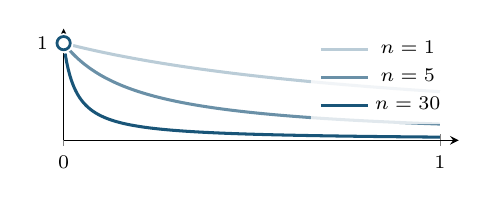
\begin{tikzpicture}
        \begin{axis}[
          width=6.6cm, height=3.0cm,
          axis lines=left,
          xmin=0, xmax=1.05, ymin=0, ymax=1.15,
          xtick={0,1}, ytick={1},
          tick label style={font=\scriptsize},
          legend style={font=\scriptsize, at={(0.99,0.99)}, anchor=north east,
            draw=none, fill=white, fill opacity=0.8, text opacity=1},
          clip=false,
        ]
          \addplot[defcolor!30, line width=1.1pt, domain=0.004:1, samples=120] {1/(x+1)};
          \addlegendentry{$n = 1$}
          \addplot[defcolor!65, line width=1.1pt, domain=0.004:1, samples=150] {1/(5*x+1)};
          \addlegendentry{$n = 5$}
          \addplot[defcolor, line width=1.1pt, domain=0.004:1, samples=250] {1/(30*x+1)};
          \addlegendentry{$n = 30$}
          \opendotpt{defcolor}{(axis cs:0,1)}
        \end{axis}
      \end{tikzpicture}
      \end{center}
    \end{column}
  \end{columns}

  \note{
    The plot shows "f" sub 1, "f" sub 5, and "f" sub 30 in increasingly
    dark blue. Each curve starts near height 1 at the left edge, marked
    by the open circle, since zero itself is excluded, and then falls
    off. As "n" grows, the fall happens closer and closer to zero, but
    it always starts at height 1. So, as the bullet says, the supremum
    of each "f" sub "n" is 1, and by Theorem 7.9 the convergence is not
    uniform. The convergence is slowest near the missing endpoint.
  }
\end{frame}

% --- Build 3/3 ---
\begin{frame}{Compactness Is Really Needed}
  \begin{exblock}{Example}
    \[
      f_n(x) = \frac{1}{nx + 1} \qquad (0 < x < 1;\ n = 1, 2, 3, \dots)
    \]
    Continuous, $f_n \geq f_{n+1}$, and $f_n(x) \to 0$ (continuous limit),
    but \alert{not uniformly}.
  \end{exblock}

  \begin{columns}[T]
    \begin{column}{0.52\textwidth}
      \begin{hlbox}
      \begin{itemize}
        \item $\sup_{(0,1)} f_n = 1$ for all $n$
        \item Bad sets $K_n = \bigl(0, \tfrac{1/\varepsilon - 1}{n}\bigr]$:
          nested, $\bigcap K_n = \varnothing$, but \alert{none is empty}
      \end{itemize}
      \end{hlbox}
    \end{column}
    \begin{column}{0.46\textwidth}
      \begin{center}
      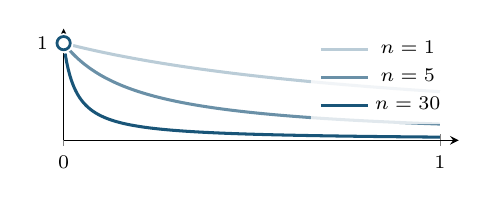
\begin{tikzpicture}
        \begin{axis}[
          width=6.6cm, height=3.0cm,
          axis lines=left,
          xmin=0, xmax=1.05, ymin=0, ymax=1.15,
          xtick={0,1}, ytick={1},
          tick label style={font=\scriptsize},
          legend style={font=\scriptsize, at={(0.99,0.99)}, anchor=north east,
            draw=none, fill=white, fill opacity=0.8, text opacity=1},
          clip=false,
        ]
          \addplot[defcolor!30, line width=1.1pt, domain=0.004:1, samples=120] {1/(x+1)};
          \addlegendentry{$n = 1$}
          \addplot[defcolor!65, line width=1.1pt, domain=0.004:1, samples=150] {1/(5*x+1)};
          \addlegendentry{$n = 5$}
          \addplot[defcolor, line width=1.1pt, domain=0.004:1, samples=250] {1/(30*x+1)};
          \addlegendentry{$n = 30$}
          \opendotpt{defcolor}{(axis cs:0,1)}
        \end{axis}
      \end{tikzpicture}
      \end{center}
    \end{column}
  \end{columns}

  \note{
    The second bullet shows exactly where the proof of Theorem 7.13
    breaks down. For epsilon between 0 and 1, the bad set capital "K"
    sub "n" is the interval from 0, excluded, up to 1 over epsilon minus
    1, all divided by "n". These sets are closed in the open interval,
    and nested, with empty intersection, just as in the proof. But they
    are not compact, since 0 is missing, and none of them is empty. So
    Theorem 2.36 has nothing to grab onto. Now let's change our point
    of view.
  }
\end{frame}
}

{
\usebackgroundtemplate{%
  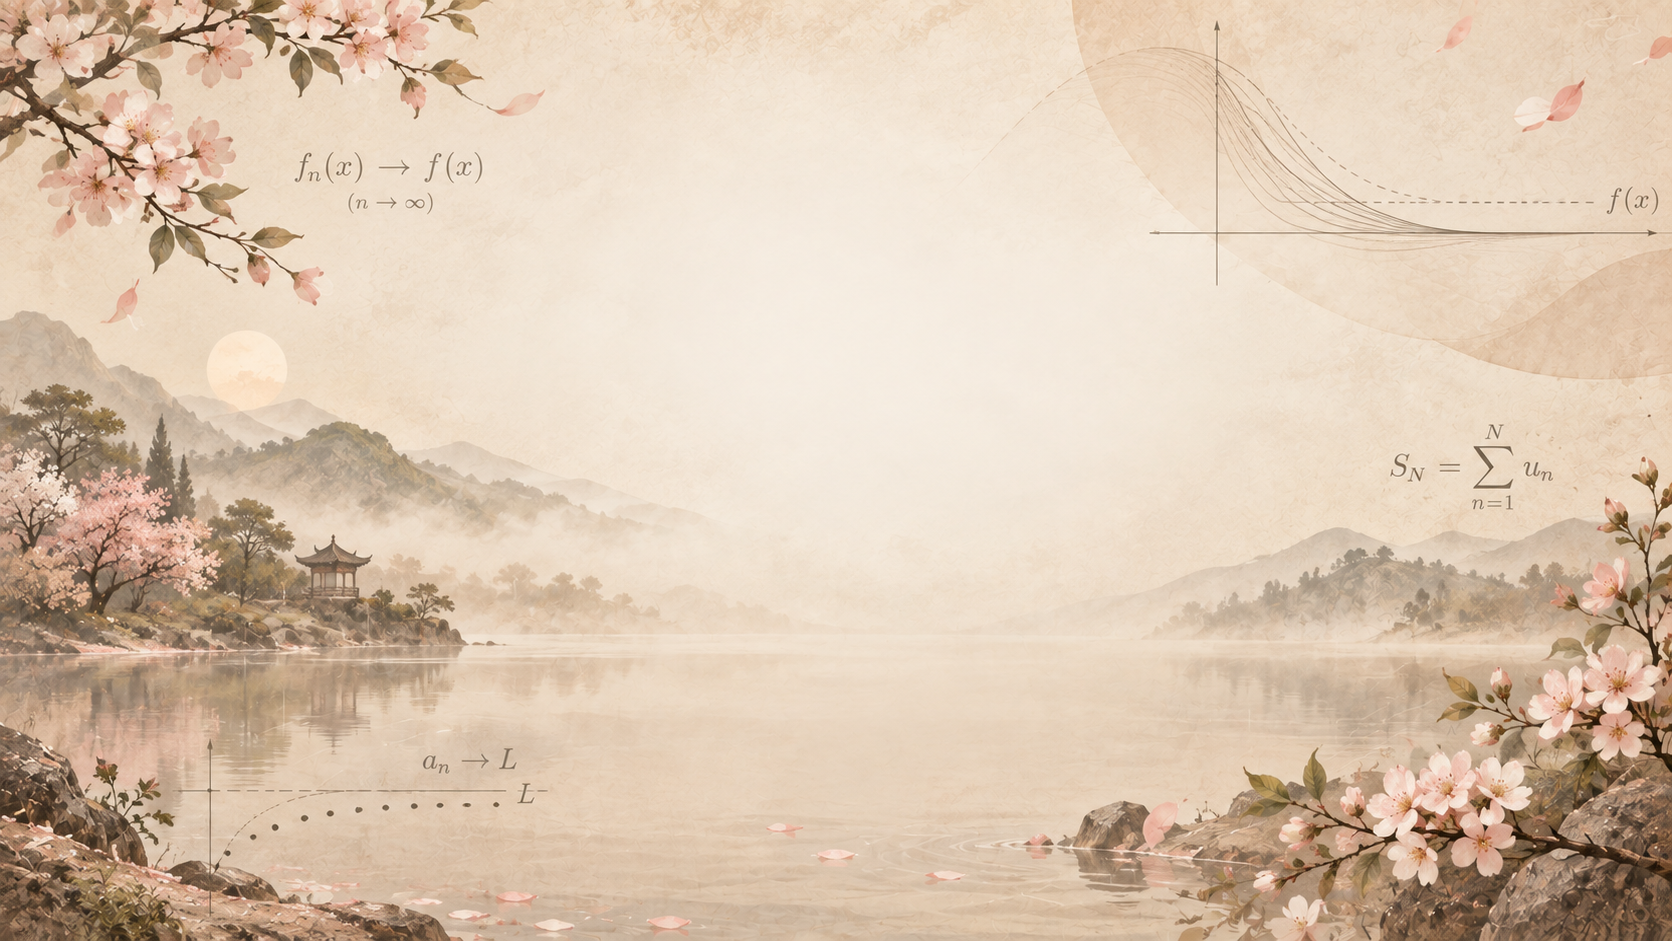
\includegraphics[width=\paperwidth,height=\paperheight,keepaspectratio=false]{chapter_07_bg_05.png}%
}
\section{The Space $\mathscr{C}(X)$}

% --- Build 1/2 ---
\begin{frame}{Definition 7.14: The Space $\mathscr{C}(X)$}
  \begin{defblock}{Definition 7.14}
    If $X$ is a metric space, $\mathscr{C}(X)$ denotes the set of all
    \alert{complex-valued, continuous, bounded} functions with domain $X$.
  \end{defblock}

  \begin{remblock}{Remark}
    If $X$ is \alert{compact}, boundedness is automatic (Theorem 4.15), so
    $\mathscr{C}(X)$ = all complex continuous functions on $X$.
  \end{remblock}

  \note{
    So far we have thought of uniform convergence as a property of a
    sequence of functions. Now we take a more geometric view, and treat
    each function as a single point in a space. Definition 7.14: for a
    metric space capital "X", script capital "C" of capital "X" is the
    set of all complex valued functions on capital "X" that are both
    continuous and bounded. The gray remark notes that when capital "X"
    is compact, boundedness is automatic, because by Theorem 4.15 a
    continuous function on a compact space is bounded. So in that case
    script capital "C" of capital "X" simply consists of all complex
    continuous functions on capital "X".
  }
\end{frame}

% --- Build 2/2 ---
\begin{frame}{Definition 7.14: The Space $\mathscr{C}(X)$}
  \begin{defblock}{Definition 7.14}
    If $X$ is a metric space, $\mathscr{C}(X)$ denotes the set of all
    \alert{complex-valued, continuous, bounded} functions with domain $X$.
  \end{defblock}

  \begin{remblock}{Remark}
    If $X$ is \alert{compact}, boundedness is automatic (Theorem 4.15), so
    $\mathscr{C}(X)$ = all complex continuous functions on $X$.
  \end{remblock}

  \begin{defblock}{Supremum norm}
    \[
      \boxed{\|f\| = \sup_{x \in X} |f(x)|} \qquad (f \in \mathscr{C}(X)).
    \]
  \end{defblock}

  \note{
    With each function "f" in script capital "C" of capital "X" we
    associate its supremum norm, written with double vertical bars: the
    supremum over all "x" of the absolute value of "f" of "x". It
    measures the size of "f" by its largest absolute value, the highest
    point the graph reaches away from zero. This is where boundedness
    is used: it guarantees the supremum is a finite number. Let's check
    the properties that make this a good measure of size.
  }
\end{frame}

% --- Build 1/3 ---
\begin{frame}{Properties of the Supremum Norm}
  \begin{hlbox}
  \begin{itemize}
    \item $\|f\| < \infty$, \ since $f$ is bounded
  \end{itemize}
  \end{hlbox}

  \note{
    First, the norm of every function in script capital "C" of capital
    "X" is a finite, nonnegative number. This is exactly why we required
    the functions to be bounded. Without boundedness, a continuous
    function such as 1 over "x" on the open unit interval would have
    infinite norm.
  }
\end{frame}

% --- Build 2/3 ---
\begin{frame}{Properties of the Supremum Norm}
  \begin{hlbox}
  \begin{itemize}
    \item $\|f\| < \infty$, \ since $f$ is bounded
    \item $\|f\| = 0$ \ only if \ $f(x) = 0$ for every $x \in X$, \ that is, $f = 0$
  \end{itemize}
  \end{hlbox}

  \note{
    Second, the norm vanishes only for the zero function. Indeed, if the
    supremum of the absolute values is zero, then every single value
    "f" of "x" has absolute value zero, so "f" is identically zero.
  }
\end{frame}

% --- Build 3/3 ---
\begin{frame}{Properties of the Supremum Norm}
  \begin{hlbox}
  \begin{itemize}
    \item $\|f\| < \infty$, \ since $f$ is bounded
    \item $\|f\| = 0$ \ only if \ $f(x) = 0$ for every $x \in X$, \ that is, $f = 0$
    \item \alert{Triangle inequality}: for $h = f + g$,
      \[
        |h(x)| \leq |f(x)| + |g(x)| \leq \|f\| + \|g\| \quad (x \in X)
        \;\Longrightarrow\; \|f + g\| \leq \|f\| + \|g\|
      \]
  \end{itemize}
  \end{hlbox}

  \note{
    Third, the triangle inequality. Let "h" be the sum of "f" and "g". At each point "x", the absolute value
    of "h" of "x" is at most the absolute value of "f" of "x" plus that
    of "g" of "x", by the triangle inequality for complex numbers. Each
    of those is at most the corresponding norm. So the right side is a
    bound that does not depend on "x", and taking the supremum over "x"
    on the left gives the boxed inequality: the norm of the sum is at
    most the sum of the norms. With these properties we can define a
    distance.
  }
\end{frame}

% --- Build 1/2 ---
\begin{frame}{$\mathscr{C}(X)$ Is a Metric Space}
  \begin{defblock}{Distance in $\mathscr{C}(X)$}
    \[
      d(f, g) = \|f - g\| = \sup_{x \in X} |f(x) - g(x)|.
    \]
    Axioms 2.15 hold $\Rightarrow$ \alert{$\mathscr{C}(X)$ is a metric space.}
  \end{defblock}

  \note{
    We define the distance between two functions "f" and "g" in script
    capital "C" of capital "X" to be the norm of their difference. The
    metric axioms from Definition 2.15 follow from what we just checked.
    The distance is finite and nonnegative, and it is zero only if "f"
    minus "g" is the zero function, that is, only if "f" equals "g". It
    is symmetric, since "f" minus "g" and "g" minus "f" have the same
    absolute values. And the triangle inequality for distances follows
    from the triangle inequality for the norm, applied to "f" minus "h"
    plus "h" minus "g". So script capital "C" of capital "X" becomes a
    metric space, whose points are functions.
  }
\end{frame}

% --- Build 2/2 ---
\begin{frame}{$\mathscr{C}(X)$ Is a Metric Space}
  \begin{defblock}{Distance in $\mathscr{C}(X)$}
    \[
      d(f, g) = \|f - g\| = \sup_{x \in X} |f(x) - g(x)|.
    \]
    Axioms 2.15 hold $\Rightarrow$ \alert{$\mathscr{C}(X)$ is a metric space.}
  \end{defblock}

  \vspace{-0.3em}
  \begin{center}
  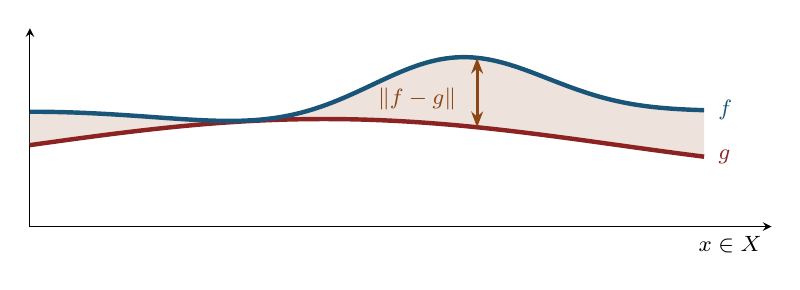
\begin{tikzpicture}
    \begin{axis}[
      width=11.0cm, height=4.1cm,
      axis lines=left,
      xmin=0, xmax=3.3, ymin=0, ymax=1.9,
      xtick=\empty, ytick=\empty,
      xlabel={$x \in X$}, xlabel style={font=\footnotesize, at={(1,0)}, anchor=north east},
      clip=false,
    ]
      \addplot[name path=gcurve, thmcolor, line width=1.6pt, domain=0:3, samples=150]
        {0.78 + 0.25*sin(deg(1.2*x))};
      \addplot[name path=fcurve, defcolor, line width=1.6pt, domain=0:3, samples=150]
        {1.0 + 0.7*exp(-3*(x-1.9)^2) + 0.1*cos(deg(2*x))};
      \addplot[mAccent!15] fill between[of=fcurve and gcurve];
      \draw[mAccent, line width=1.1pt, {Stealth[length=2mm]}-{Stealth[length=2mm]}]
        (axis cs:1.99,0.951) -- (axis cs:1.99,1.616);
      \node[mAccent, font=\footnotesize, anchor=east] at (axis cs:1.94,1.22) {$\|f - g\|$};
      \node[defcolor, font=\footnotesize, anchor=west] at (axis cs:3.02,1.115) {$f$};
      \node[thmcolor, font=\footnotesize, anchor=west] at (axis cs:3.02,0.669) {$g$};
    \end{axis}
  \end{tikzpicture}
  \end{center}

  \note{
    The picture shows what this distance means. The blue curve is "f",
    the red curve is "g", and the light orange shading fills the region
    between them. The distance between "f" and "g" is the largest
    vertical gap between the two graphs, marked by the orange double
    arrow, labeled on its left, at the point where the blue bump rises
    highest above the red curve. Two functions are close in this metric only if their graphs
    are close everywhere at once, not just at some points.
  }
\end{frame}

% --- Build 1/2 ---
\begin{frame}{Convergence in $\mathscr{C}(X)$ = Uniform Convergence}
  \begin{thmblock}{Theorem 7.9, rephrased}
    \[
      f_n \to f \text{ in the metric of } \mathscr{C}(X)
      \quad\iff\quad
      f_n \to f \text{ \alert{uniformly} on } X.
    \]
  \end{thmblock}

  \note{
    Here is the payoff of the new viewpoint. Recall Theorem 7.9: a
    sequence converges uniformly exactly when the supremum of the
    distance between "f" sub "n" and "f" tends to zero. But that
    supremum is precisely the distance between "f" sub "n" and "f" in
    script capital "C" of capital "X". So convergence in this metric
    space is the same thing as uniform convergence. The epsilon tube
    around "f" from the previous section is nothing but the closed ball
    of radius epsilon around the point "f".
  }
\end{frame}

% --- Build 2/2 ---
\begin{frame}{Convergence in $\mathscr{C}(X)$ = Uniform Convergence}
  \begin{thmblock}{Theorem 7.9, rephrased}
    \[
      f_n \to f \text{ in the metric of } \mathscr{C}(X)
      \quad\iff\quad
      f_n \to f \text{ \alert{uniformly} on } X.
    \]
  \end{thmblock}

  \vspace{0.3em}
  \begin{defblock}{Terminology}
    \begin{itemize}
      \item Closed subsets of $\mathscr{C}(X)$: \alert{uniformly closed}
      \item Closure of $\mathscr{A} \subset \mathscr{C}(X)$: its \alert{uniform closure}
    \end{itemize}
  \end{defblock}

  \note{
    Accordingly, topological words in script capital "C" of capital "X"
    get the adjective uniform. A closed subset of script capital "C" of
    capital "X" is called uniformly closed: it contains all uniform
    limits of its members. And the closure of a set of functions, say
    script capital "A", is called its uniform closure: it consists of
    all functions that can be uniformly approximated by members of
    script capital "A". This language will be central at the end of the
    chapter, in the Stone Weierstrass theorem, which describes the
    uniform closure of the polynomials. One more theorem remains.
  }
\end{frame}
}

{
\usebackgroundtemplate{%
  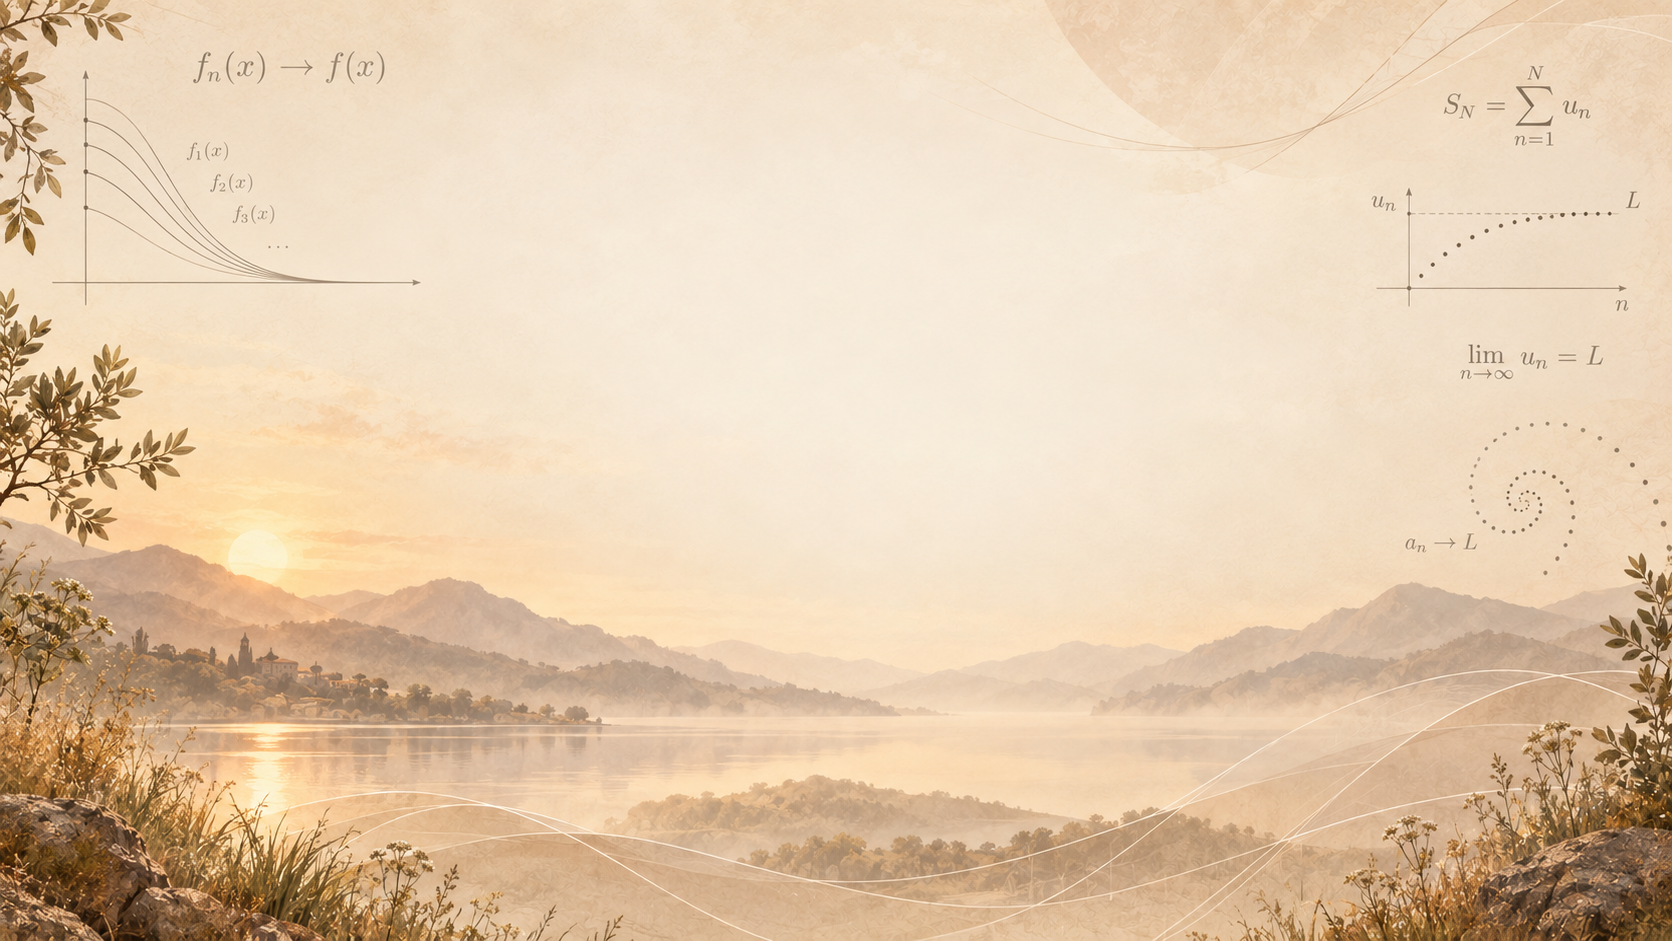
\includegraphics[width=\paperwidth,height=\paperheight,keepaspectratio=false]{chapter_07_bg_06.png}%
}
\section{Completeness of $\mathscr{C}(X)$}

% --- Build 1/2 ---
\begin{frame}{Theorem 7.15: $\mathscr{C}(X)$ Is Complete}
  \begin{thmblock}{Theorem 7.15}
    The above metric makes $\mathscr{C}(X)$ into a \alert{complete} metric space.
  \end{thmblock}

  \note{
    Theorem 7.15 says that script capital "C" of capital "X", with the
    supremum metric, is complete: every Cauchy sequence converges to a
    point of the space. Recall that the rationals lack this property,
    while the reals and the Euclidean spaces have it. Completeness is
    what makes a space good for analysis: to prove that a limit exists,
    it is enough to show that the terms get close to each other.
  }
\end{frame}

% --- Build 2/2 ---
\begin{frame}{Theorem 7.15: $\mathscr{C}(X)$ Is Complete}
  \begin{thmblock}{Theorem 7.15}
    The above metric makes $\mathscr{C}(X)$ into a \alert{complete} metric space.
  \end{thmblock}

  \vspace{0.6em}
  \begin{hlbox}
  \textbf{Strategy:} Take a Cauchy sequence $\{f_n\}$ in $\mathscr{C}(X)$.
  \begin{enumerate}
    \item Find a \alert{uniform} limit $f$ \hfill (Theorem 7.8)
    \item Show $f$ is \alert{continuous} \hfill (Theorem 7.12)
    \item Show $f$ is \alert{bounded}
    \item Conclude $f \in \mathscr{C}(X)$ and $\|f - f_n\| \to 0$
  \end{enumerate}
  \end{hlbox}

  \note{
    The strategy has four steps. Given a Cauchy sequence of functions,
    we first produce a uniform limit using the Cauchy criterion, Theorem
    7.8. Second, the limit is continuous by Theorem 7.12, which we
    proved earlier in this section. Third, the limit is bounded. And
    finally, we conclude that it belongs to the space and that the
    sequence converges to it in the metric. Let's carry this out.
  }
\end{frame}

% --- Build 1/2 ---
\begin{frame}{Proof of Theorem 7.15}
  \begin{proofblock}{Step 1: A uniform limit exists}
    $\{f_n\}$ Cauchy in $\mathscr{C}(X)$: for each $\varepsilon > 0$ there is $N$ with
    \[
      \|f_n - f_m\| < \varepsilon \quad (n, m \geq N),
      \ \text{ i.e. } |f_n(x) - f_m(x)| < \varepsilon \ \ \forall x \in X.
    \]
    By Theorem 7.8, $f_n \to f$ \alert{uniformly} for some $f : X \to \mathbb{C}$.
  \end{proofblock}

  \note{
    Let "f" sub "n" be a Cauchy sequence in script capital "C" of capital
    "X". By the definition of the metric, this means that for every
    epsilon there is a capital "N" such that the norm of "f" sub "n"
    minus "f" sub "m" is less than epsilon for all indices beyond
    capital "N". Unpacking the supremum, the values "f" sub "n" of "x"
    and "f" sub "m" of "x" are within epsilon of each other at every
    point "x" at once. That is exactly the Cauchy condition of Theorem
    7.8, so there is a function "f" on capital "X" to which "f" sub "n"
    converges uniformly. At this stage we only know that "f" is some
    complex function; we still need to show it lies in our space.
  }
\end{frame}

% --- Build 2/2 ---
\begin{frame}{Proof of Theorem 7.15}
  \begin{proofblock}{Step 1: A uniform limit exists}
    $\{f_n\}$ Cauchy in $\mathscr{C}(X)$: for each $\varepsilon > 0$ there is $N$ with
    \[
      \|f_n - f_m\| < \varepsilon \quad (n, m \geq N),
      \ \text{ i.e. } |f_n(x) - f_m(x)| < \varepsilon \ \ \forall x \in X.
    \]
    By Theorem 7.8, $f_n \to f$ \alert{uniformly} for some $f : X \to \mathbb{C}$.
  \end{proofblock}
  \begin{proofblock}{Steps 2--4: $f \in \mathscr{C}(X)$ and $f_n \to f$ in the metric}
    \begin{itemize}
      \item $f$ \alert{continuous}: Theorem 7.12
      \item $f$ \alert{bounded}: pick $n$ with $|f - f_n| < 1$ on $X$; then
        $|f| < \|f_n\| + 1$
      \item $f \in \mathscr{C}(X)$ and, by uniform convergence, $\|f - f_n\| \to 0$.
        \hfill $\blacksquare$
    \end{itemize}
  \end{proofblock}

  \note{
    The remaining steps are short. Since each "f" sub "n" is continuous
    and the convergence is uniform, Theorem 7.12 says "f" is continuous.
    For boundedness, uniform convergence with epsilon equal to 1 gives
    an index "n" such that "f" is within 1 of "f" sub "n" at every
    point. Since "f" sub "n" is bounded by its norm, "f" is bounded by
    that norm plus 1. So "f" is continuous and bounded, which means it
    is a point of script capital "C" of capital "X". Finally, uniform
    convergence is the same as convergence in the metric, so the norm
    of "f" minus "f" sub "n" tends to zero. Every Cauchy sequence
    converges, and the space is complete.
  }
\end{frame}
}

{
\usebackgroundtemplate{%
  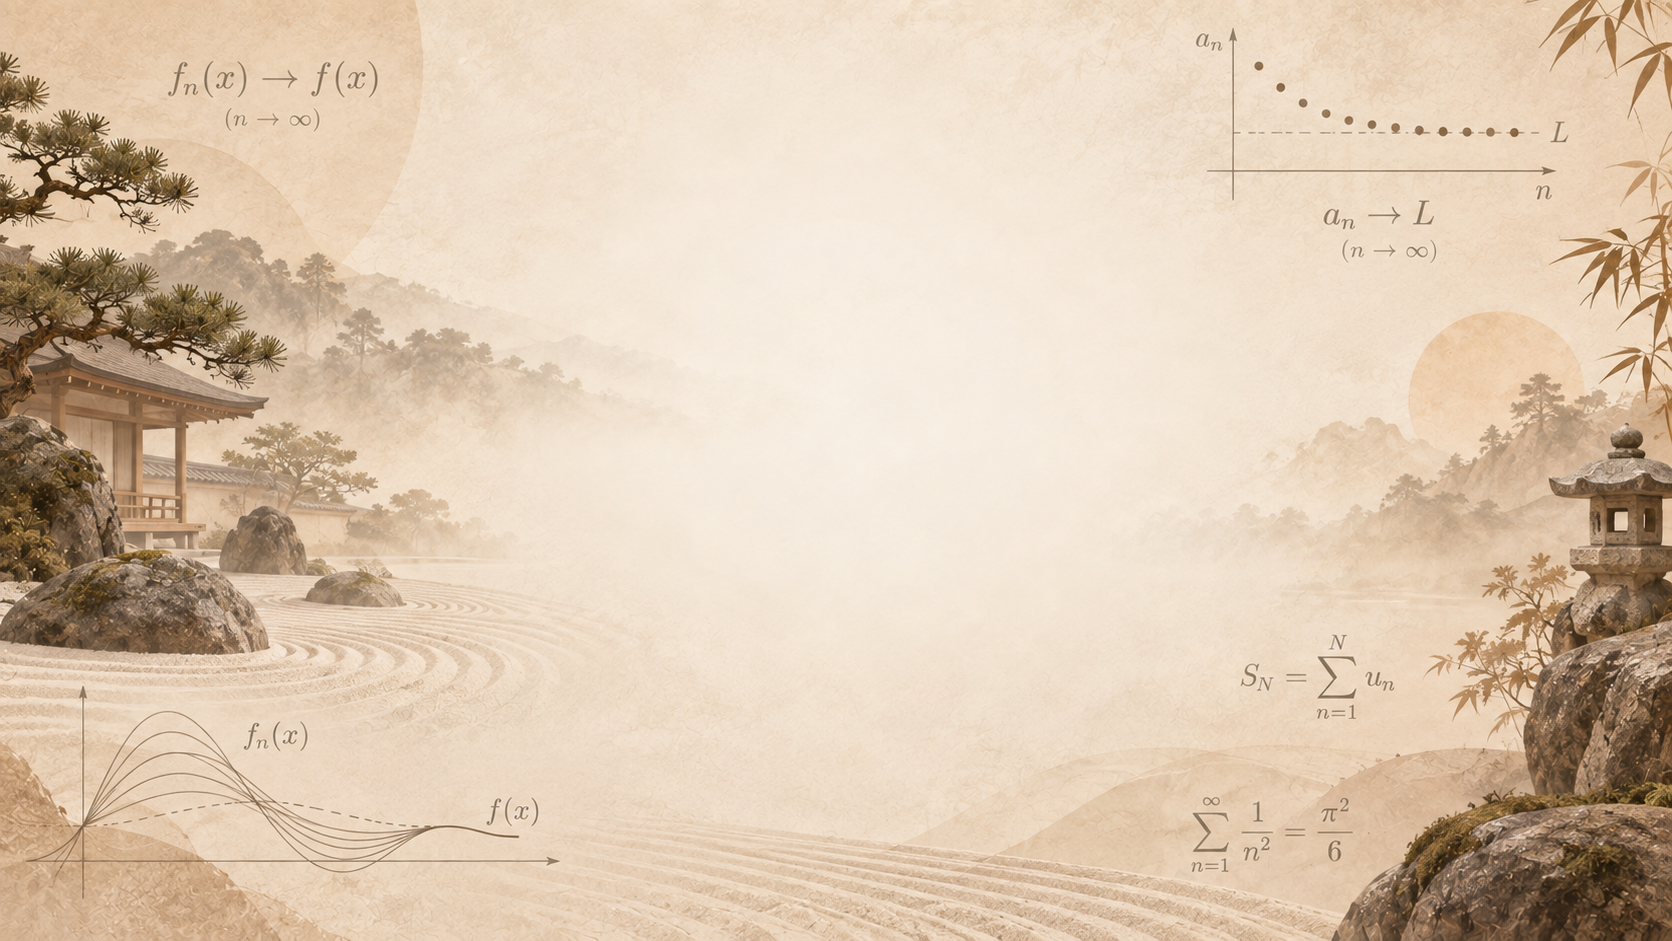
\includegraphics[width=\paperwidth,height=\paperheight,keepaspectratio=false]{chapter_07_bg_07.png}%
}
\section{Summary}

% --- Build 1/4 ---
\begin{frame}{Summary}
  \begin{hlbox}
  \textbf{Key takeaways from this section:}
  \begin{itemize}
    \item \textbf{Theorem 7.11:} uniform $\Rightarrow$
      $\lim_{t \to x} \lim_{n \to \infty} f_n(t)
      = \lim_{n \to \infty} \lim_{t \to x} f_n(t)$
  \end{itemize}
  \end{hlbox}

  \note{
    Let's review. Theorem 7.11 showed that under uniform convergence
    the limit in "t" and the limit in "n" can be interchanged. The
    proof was an epsilon over 3 argument, and its key point was that
    uniformity allowed us to fix one index "n" before choosing the point
    "t". Next, continuity.
  }
\end{frame}

% --- Build 2/4 ---
\begin{frame}{Summary}
  \begin{hlbox}
  \textbf{Key takeaways from this section:}
  \begin{itemize}
    \item \textbf{Theorem 7.11:} uniform $\Rightarrow$
      $\lim_{t \to x} \lim_{n \to \infty} f_n(t)
      = \lim_{n \to \infty} \lim_{t \to x} f_n(t)$
    \item \textbf{Theorem 7.12:} uniform limit of continuous is \alert{continuous};
      converse false (Ex.\ 7.6)
  \end{itemize}
  \end{hlbox}

  \note{
    Theorem 7.12, the main result, followed at once: a uniform limit of
    continuous functions is continuous. This settles the main problem
    for continuity, and it also serves as a test: a discontinuous limit
    of continuous functions, as with the powers of "x", signals non
    uniform convergence. The converse fails, as Example 7.6 showed with
    its growing bumps. Next, the partial converse.
  }
\end{frame}

% --- Build 3/4 ---
\begin{frame}{Summary}
  \begin{hlbox}
  \textbf{Key takeaways from this section:}
  \begin{itemize}
    \item \textbf{Theorem 7.11:} uniform $\Rightarrow$
      $\lim_{t \to x} \lim_{n \to \infty} f_n(t)
      = \lim_{n \to \infty} \lim_{t \to x} f_n(t)$
    \item \textbf{Theorem 7.12:} uniform limit of continuous is \alert{continuous};
      converse false (Ex.\ 7.6)
    \item \textbf{Theorem 7.13 (Dini):} \alert{compact} $K$, continuous
      $f_n \downarrow f$ continuous $\Rightarrow$ uniform
  \end{itemize}
  \end{hlbox}

  \note{
    Theorem 7.13, known as Dini's theorem, is a partial converse: on a
    compact set, a decreasing sequence of continuous functions with a
    continuous pointwise limit converges uniformly. The proof used
    nested compact bad sets, and the example of 1 over "n" "x" plus 1
    on the open interval showed that compactness cannot be dropped.
    Finally, the space of functions.
  }
\end{frame}

% --- Build 4/4 ---
\begin{frame}{Summary}
  \begin{hlbox}
  \textbf{Key takeaways from this section:}
  \begin{itemize}
    \item \textbf{Theorem 7.11:} uniform $\Rightarrow$
      $\lim_{t \to x} \lim_{n \to \infty} f_n(t)
      = \lim_{n \to \infty} \lim_{t \to x} f_n(t)$
    \item \textbf{Theorem 7.12:} uniform limit of continuous is \alert{continuous};
      converse false (Ex.\ 7.6)
    \item \textbf{Theorem 7.13 (Dini):} \alert{compact} $K$, continuous
      $f_n \downarrow f$ continuous $\Rightarrow$ uniform
    \item \textbf{7.14--7.15:} $\mathscr{C}(X)$, $\|f\| = \sup |f|$: \alert{complete};
      convergence = uniform
  \end{itemize}

  \vspace{0.2em}
  \textbf{Coming up next:} uniform convergence and \alert{integration}.
  \end{hlbox}

  \note{
    Definition 7.14 introduced script capital "C" of capital "X", the
    continuous bounded functions with the supremum norm. Convergence in
    this metric is exactly uniform convergence, and Theorem 7.15 showed
    the space is complete. In the next section, Uniform Convergence and
    Integration, we turn to the second part of the main problem, and
    show that uniform convergence also allows us to interchange limits
    and integrals, which failed in Example 7.6. See you next time.
  }
\end{frame}
}

\end{document}
